% !Mode:: "TeX:UTF-8"
\chapter{系统实现与功能展示}

\section{开发环境与工具配置}

本系统的开发、测试和部署涉及前端、业务后端、算法后端和底层物理执行四个层面。
为了让系统实现和后续实验环境保持一致，
本章和第六章采用同一套软硬件配置。
表\ref{tab:dev_env}列出系统实现和实验验证所使用的主要环境配置。

\begin{table}[htbp]
\centering
\caption{开发环境与工具配置清单}
\label{tab:dev_env}
\small
\begin{tabular}{>{\raggedright\arraybackslash}p{2.1cm}>{\raggedright\arraybackslash}p{3.9cm}>{\raggedright\arraybackslash}p{2.7cm}>{\raggedright\arraybackslash}p{3.8cm}}
\toprule
类别 & 名称 & 版本/规格 & 用途 \\
\midrule
操作系统 & Windows 11 + WSL2 (Ubuntu 22.04) & 23H2 & 开发与物理执行 \\
处理器 & Intel Core i7-12700H & 14核20线程 & 编译与实验运行 \\
内存 & DDR4 & 16\,GB & 数据导入与服务运行 \\
显卡 & NVIDIA RTX 3060 Laptop GPU & 6\,GB GDDR6 & CUDA算子执行 \\
CUDA工具链 & CUDA Toolkit & 11.8 & GPU运行时环境 \\
前端框架 & Vue 3 + TypeScript & 3.3 / 5.3 & 单页应用开发 \\
UI组件库 & Element Plus & 2.4 & 界面组件渲染 \\
构建工具 & Vite & 5.0 & 前端热更新打包 \\
业务后端 & Java Spring Boot + JPA/Hibernate & 3.2 / 8080端口 & 结构化数据管理与代理转发 \\
JDK & OpenJDK & 17 & Java运行时 \\
算法后端 & Python FastAPI & 0.104 / 5000端口 & 算法服务与RAG \\
Python & CPython & 3.11 & 算法后端运行时 \\
关系数据库 & MySQL & 8.0 & 结构化元数据存储 \\
向量数据库 & Milvus & 2.3.x & 高维语义向量存储 \\
语义编码 & all-MiniLM-L6-v2 & 384维输出 & 日志与脚本结构向量化 \\
深度学习框架 & PyTorch & 2.1.0源码编译 & 物理执行与覆盖率采集 \\
覆盖率工具 & Gcov / LCOV & GCC 11 / 1.16 & C++层探针采集 \\
前端图表 & ECharts & --- & 散点图、热力图与统计图表展示 \\
\bottomrule
\end{tabular}
\end{table}

当前实现中，
前端运行在Vite开发服务器上（默认端口5173），
通过Axios访问Java Spring Boot后端和Python FastAPI后端。
Java后端（端口8080）主要负责结构化数据管理与部分代理转发，
Python后端（端口5000）主要负责语义检索、候选边界条件分析、
CEI分析和候选补盲建议等算法处理。

底层物理执行环境部署在WSL2中的Ubuntu 22.04子系统里。
这个子系统里安装了带Gcov探针的PyTorch编译版本，
以及独立的Python虚拟环境\texttt{venv\_pytorch}。
物理执行层通过\texttt{multiprocessing}模块的\texttt{spawn}启动方式创建独立的子进程，
在WSL环境下调用插桩后的PyTorch库执行测试脚本，
采集覆盖贡献数据。

\section{后端主要模块实现}

\subsection{Python FastAPI算法后端实现}

Python FastAPI算法后端主要负责语义编码、向量检索、PCA降维、Daikon候选边界条件分析和RAG相关接口。
服务初始化阶段建立Milvus连接、
加载两个向量集合及Sentence-BERT编码模型；
MySQL连接则在处理具体请求时按需建立。

该后端注册了数据导入、语义检索、统计分析、候选边界条件分析、CEI清退和补盲建议等API路由。
表\ref{tab:api_routes}列出主要路由的方法、路径和功能摘要。

\begin{table}[htbp]
\centering
\setlength{\tabcolsep}{6pt}
\renewcommand{\arraystretch}{1.4}
\caption{Python FastAPI算法后端API路由清单}
\label{tab:api_routes}
\begin{tabular}{llp{7.1cm}}
\toprule
方法 & 路径 & 功能摘要 \\
\midrule
POST & \texttt{/api/ingest} & 批量导入测试用例，执行双路向量化与写入 \\
POST & \texttt{/api/search} & 语义检索并返回匹配用例 \\
POST & \texttt{/api/ask} & RAG辅助诊断问答 \\
GET & \texttt{/api/recent\_cases} & 获取最近入库的测试用例列表 \\
GET & \texttt{/api/statistics} & 全局统计概览 \\
GET & \texttt{/api/analysis/}\allowbreak\texttt{coverage-gaps} & 算子覆盖热力图与覆盖缺口统计 \\
GET & \texttt{/api/analysis/}\allowbreak\texttt{efficiency} & CEI效能统计与散点分布 \\
GET & \texttt{/api/analysis/}\allowbreak\texttt{error-patterns} & 错误模式交叉聚类分析 \\
GET & \texttt{/api/analysis/}\allowbreak\texttt{correlations} & 算子-错误关联矩阵 \\
POST & \texttt{/api/analysis/}\allowbreak\texttt{fault-boundary} & 候选边界条件分析与辅助诊断报告生成 \\
POST & \texttt{/api/suggest} & 基于历史数据的变异建议生成 \\
POST & \texttt{/api/auto-generate}\allowbreak\texttt{-from-gaps} & 覆盖盲区候选补盲测试脚本生成 \\
POST & \texttt{/api/analysis/}\allowbreak\texttt{efficiency/prune} & CEI阈值清退预览与执行 \\
\bottomrule
\end{tabular}
\end{table}

语义检索接口\texttt{/api/search}的请求体以\texttt{query}字段为核心，
用于接收自然语言查询文本。
请求模型还包含\texttt{top\_k}、\texttt{search\_mode}、
\texttt{structure\_weight}和\texttt{log\_weight}等字段，
用于描述检索模式和结构向量与日志向量的融合权重；
响应体包含\texttt{total}、\texttt{results}、\texttt{query}、
\texttt{search\_mode}和\texttt{query\_intent}等字段，
其中\texttt{results}数组保存匹配用例及其相似度得分。

候选边界条件分析接口\texttt{/api/analysis/fault-boundary}的请求体包含
\texttt{failed\_case\_uid}字段，
用于指定待分析的崩溃用例。
响应体包含\texttt{failed\_case}、\texttt{successful\_case}、
\texttt{diff}、\texttt{batch\_context}、\texttt{daikon\_violations}、
\texttt{daikon\_validation}和\texttt{boundary\_rule}等字段。
其中，\texttt{diff}用于展示参数差异，
\texttt{daikon\_validation}保存待人工验证的正反样例，
\texttt{boundary\_rule}保存辅助诊断报告。

\subsection{Java Spring Boot业务后端实现}

Java Spring Boot后端承担基础业务数据管理和前端请求组织功能，
监听8080端口，并通过Spring Data JPA与MySQL交互。
该后端提供的主要API路由如表\ref{tab:java_api_routes}所示。

\begin{table}[htbp]
\centering
\setlength{\tabcolsep}{6pt}
\renewcommand{\arraystretch}{1.25}
\caption{Java Spring Boot业务后端API路由清单}
\label{tab:java_api_routes}
\begin{tabular}{llp{7.1cm}}
\toprule
方法 & 路径 & 功能摘要 \\
\midrule
GET & \texttt{/api/cases} & 分页查询测试用例，可按状态过滤 \\
GET & \texttt{/api/cases/recent} & 获取最近测试用例，用于运行总览展示 \\
GET & \texttt{/api/cases/\{id\}} & 按物理主键查询单个测试用例 \\
GET & \texttt{/api/cases/uid/}\allowbreak\texttt{\{caseUid\}} & 按业务标识符查询单个测试用例 \\
GET & \texttt{/api/statistics/}\allowbreak\texttt{overview} & 返回总数、崩溃数、平均耗时和平均覆盖数据 \\
GET & \texttt{/api/statistics/}\allowbreak\texttt{status} & 返回不同状态的用例数量 \\
GET & \texttt{/api/statistics/}\allowbreak\texttt{errors} & 返回错误类型排行 \\
POST & \texttt{/api/search} & 代理语义检索请求到Python服务 \\
POST & \texttt{/api/ask} & 代理RAG辅助诊断请求到Python服务 \\
\bottomrule
\end{tabular}
\end{table}

其中，统计接口组包含三条路由：
\texttt{/api/statistics/overview}返回用例总数、崩溃率和平均执行耗时；
\texttt{/api/statistics/status}返回各状态类别的用例数；
\texttt{/api/statistics/errors}返回错误类型。
这些结果会被封装为前端图表组件可以直接使用的JSON格式。

对语义检索和RAG辅助诊断请求，
Java后端通过Spring Cloud OpenFeign转发到配置项
\texttt{python-service.url}对应的Python服务，
再把响应体返回给前端。

\subsection{数据库表结构与向量集合详细设计}

表\texttt{test\_case\_metadata}
负责存储测试用例结构化元数据。
表\ref{tab:mysql_schema}列出了该表的完整字段设计。

\begin{table}[htbp]
\centering
\caption{MySQL主要表test\_case\_metadata字段设计}
\label{tab:mysql_schema}
\begin{tabular}{llcp{5.5cm}}
\toprule
字段名 & 数据类型 & 主键 & 说明 \\
\midrule
\texttt{id} & BIGINT & 是 & 自增物理主键 \\
\texttt{case\_uid} & VARCHAR(64) & 唯一 & 全局唯一业务标识符 \\
\texttt{status} & VARCHAR(20) & --- & 执行状态（Success/Crash/\allowbreak{}Timeout） \\
\texttt{edge\_coverage} & INT & --- & Gcov采集的分支边覆盖数 \\
\texttt{execution\_time} & FLOAT & --- & 执行耗时（秒） \\
\texttt{error\_message} & TEXT & --- & 原始崩溃日志文本 \\
\texttt{vector\_id} & BIGINT & --- & Milvus结构向量集合中的主键 \\
\texttt{parameters} & JSON & --- & 扩展信息（模型结构、双向量ID、\allowbreak{}PCA坐标等） \\
\texttt{created\_at} & DATETIME & --- & 记录创建时间戳 \\
\texttt{updated\_at} & DATETIME & --- & 记录最后更新时间戳 \\
\bottomrule
\end{tabular}
\end{table}

在\texttt{case\_uid}字段上建立唯一索引，
通过\texttt{ON DUPLICATE KEY UPDATE}语义在重复导入时更新已有记录。
\texttt{parameters}字段采用JSON类型，
保存模型结构字典、PCA降维坐标和Milvus双向量主键等扩展信息。
其中Milvus双向量主键包括\texttt{structure\_vector\_id}和\texttt{log\_vector\_id}。

Milvus侧维护两个独立的向量集合，Schema配置相同。
表\ref{tab:milvus_schema}列出了集合的字段与索引参数。

\begin{table}[htbp]
\centering
\caption{Milvus向量集合Schema与索引配置}
\label{tab:milvus_schema}
\begin{tabular}{lll}
\toprule
配置项 & 参数 & 值 \\
\midrule
集合名称（结构向量） & --- & \texttt{fuzzing\_structure} \\
集合名称（日志向量） & --- & \texttt{fuzzing\_logs} \\
主键字段 & \texttt{id} & INT64，自动生成 \\
向量字段 & \texttt{embedding} & FLOAT\_VECTOR，维度384 \\
索引类型 & \texttt{index\_type} & IVF\_FLAT \\
相似度度量 & \texttt{metric\_type} & COSINE \\
倒排列表数量 & \texttt{nlist} & 128 \\
检索探测簇数 & \texttt{nprobe} & 16 \\
\bottomrule
\end{tabular}
\end{table}

两个集合在服务启动时执行\texttt{collection.load()}操作，
把索引结构和向量数据加载到Milvus的查询节点内存中，
从而降低检索请求触发额外加载的开销。

跨库数据关联通过写入顺序和主键回填共同维护：
结构向量主键写入\texttt{vector\_id}字段，
\texttt{structure\_vector\_id}和\texttt{log\_vector\_id}
写入\texttt{parameters} JSON字段。
清退时，系统先删除Milvus中的对应向量，
再删除MySQL中的元数据记录。

\section{前端界面实现与功能展示}

本系统前端采用Vue 3和TypeScript实现，
界面组件主要基于Element Plus搭建。
页面整体以深色风格为主，
通过卡片、表格、弹窗等形式展示测试用例、统计结果和分析信息。
在实现上，前端按页面功能发起HTTP请求，
其中用例管理和基础统计主要访问Java后端，
数据导入、故障分析和补盲建议等功能则调用Python后端接口。

\subsection{FuzzHub运行总览}

FuzzHub运行总览是用户进入系统后的首页，
主要用于查看测试任务的整体情况。
页面上方用统计卡片展示累计用例数、通过率、崩溃总数和平均执行耗时，
中部展示测试状态分布，
底部列出最近产生的测试用例。
通过该页面，用户可以先对当前测试集的规模、失败比例和近期执行情况有一个整体认识。
FuzzHub运行总览界面如图\ref{fig:ui_dashboard}所示。

\begin{figure}[htbp]
\centering
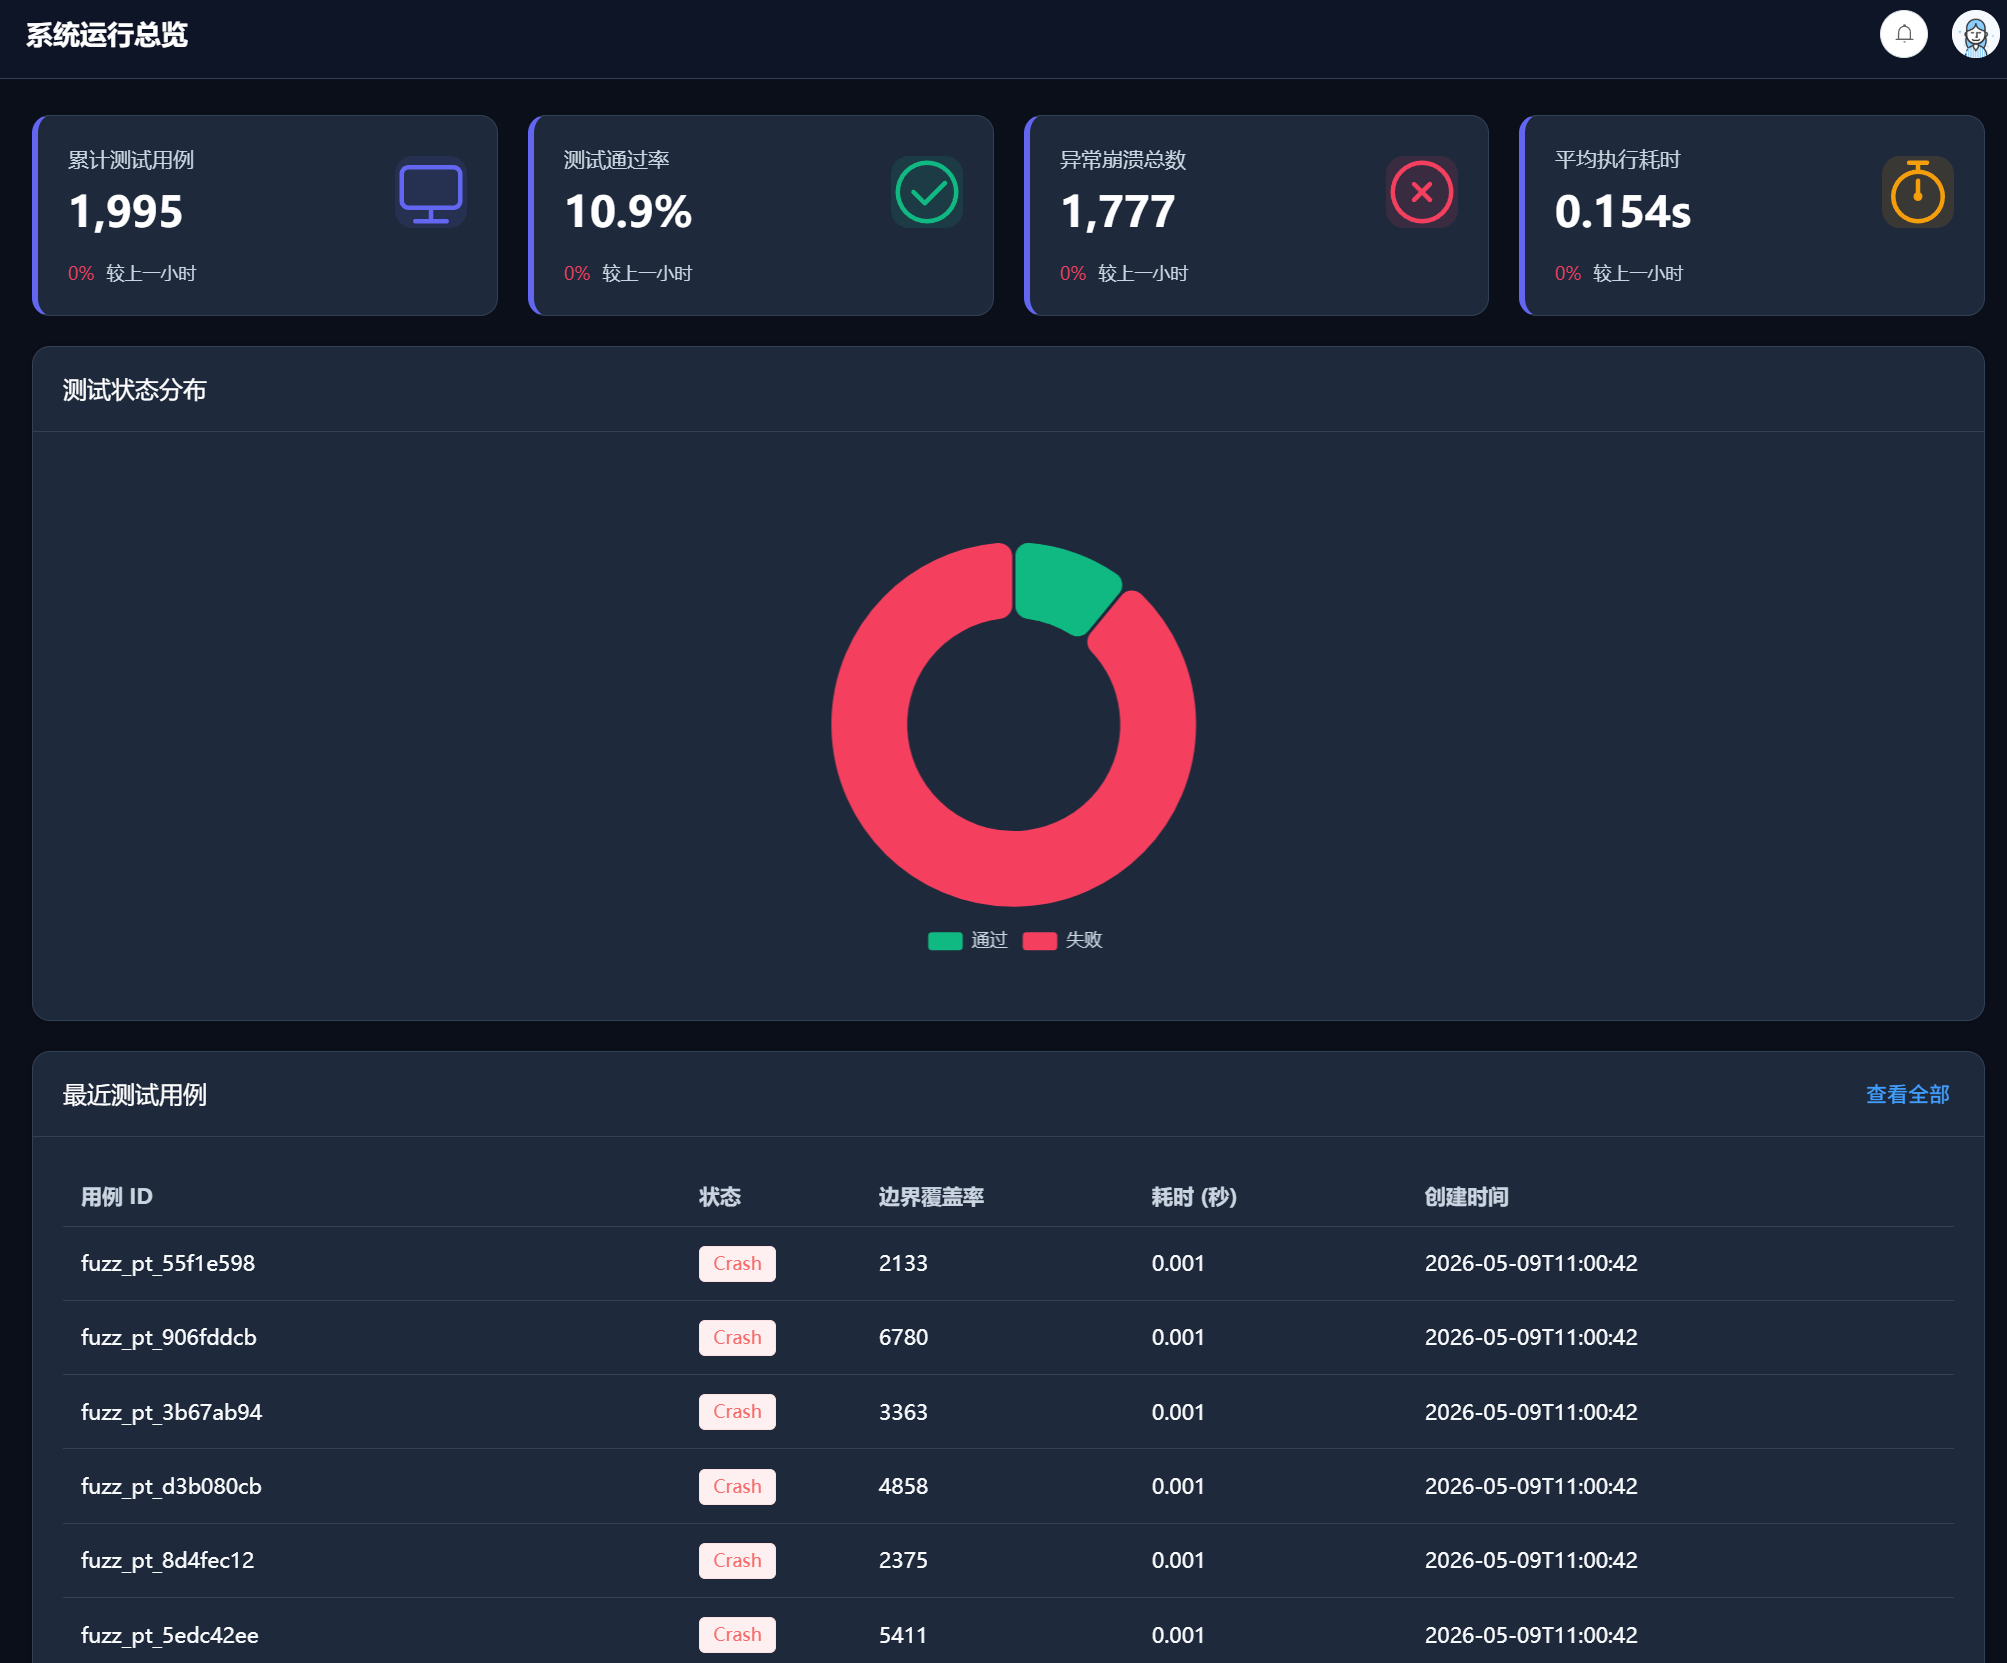
\includegraphics[width=0.75\textwidth]{figure/ui_dashboard.png}
\caption{FuzzHub运行总览界面}
\label{fig:ui_dashboard}
\end{figure}

\subsection{用例管理界面}

用例管理页面用于浏览和筛选测试用例。
用户可以按照执行状态、用例编号等条件查看记录，
也可以进入单条用例的详情页面。
表格中主要展示用例ID、执行状态、覆盖数据、运行耗时和错误摘要等信息。
该页面承担了测试数据入口的作用，
便于用户从大量用例中快速找到需要进一步分析的失败样例。
测试用例管理界面如图\ref{fig:ui_sample_manage}所示。

\begin{figure}[htbp]
\centering
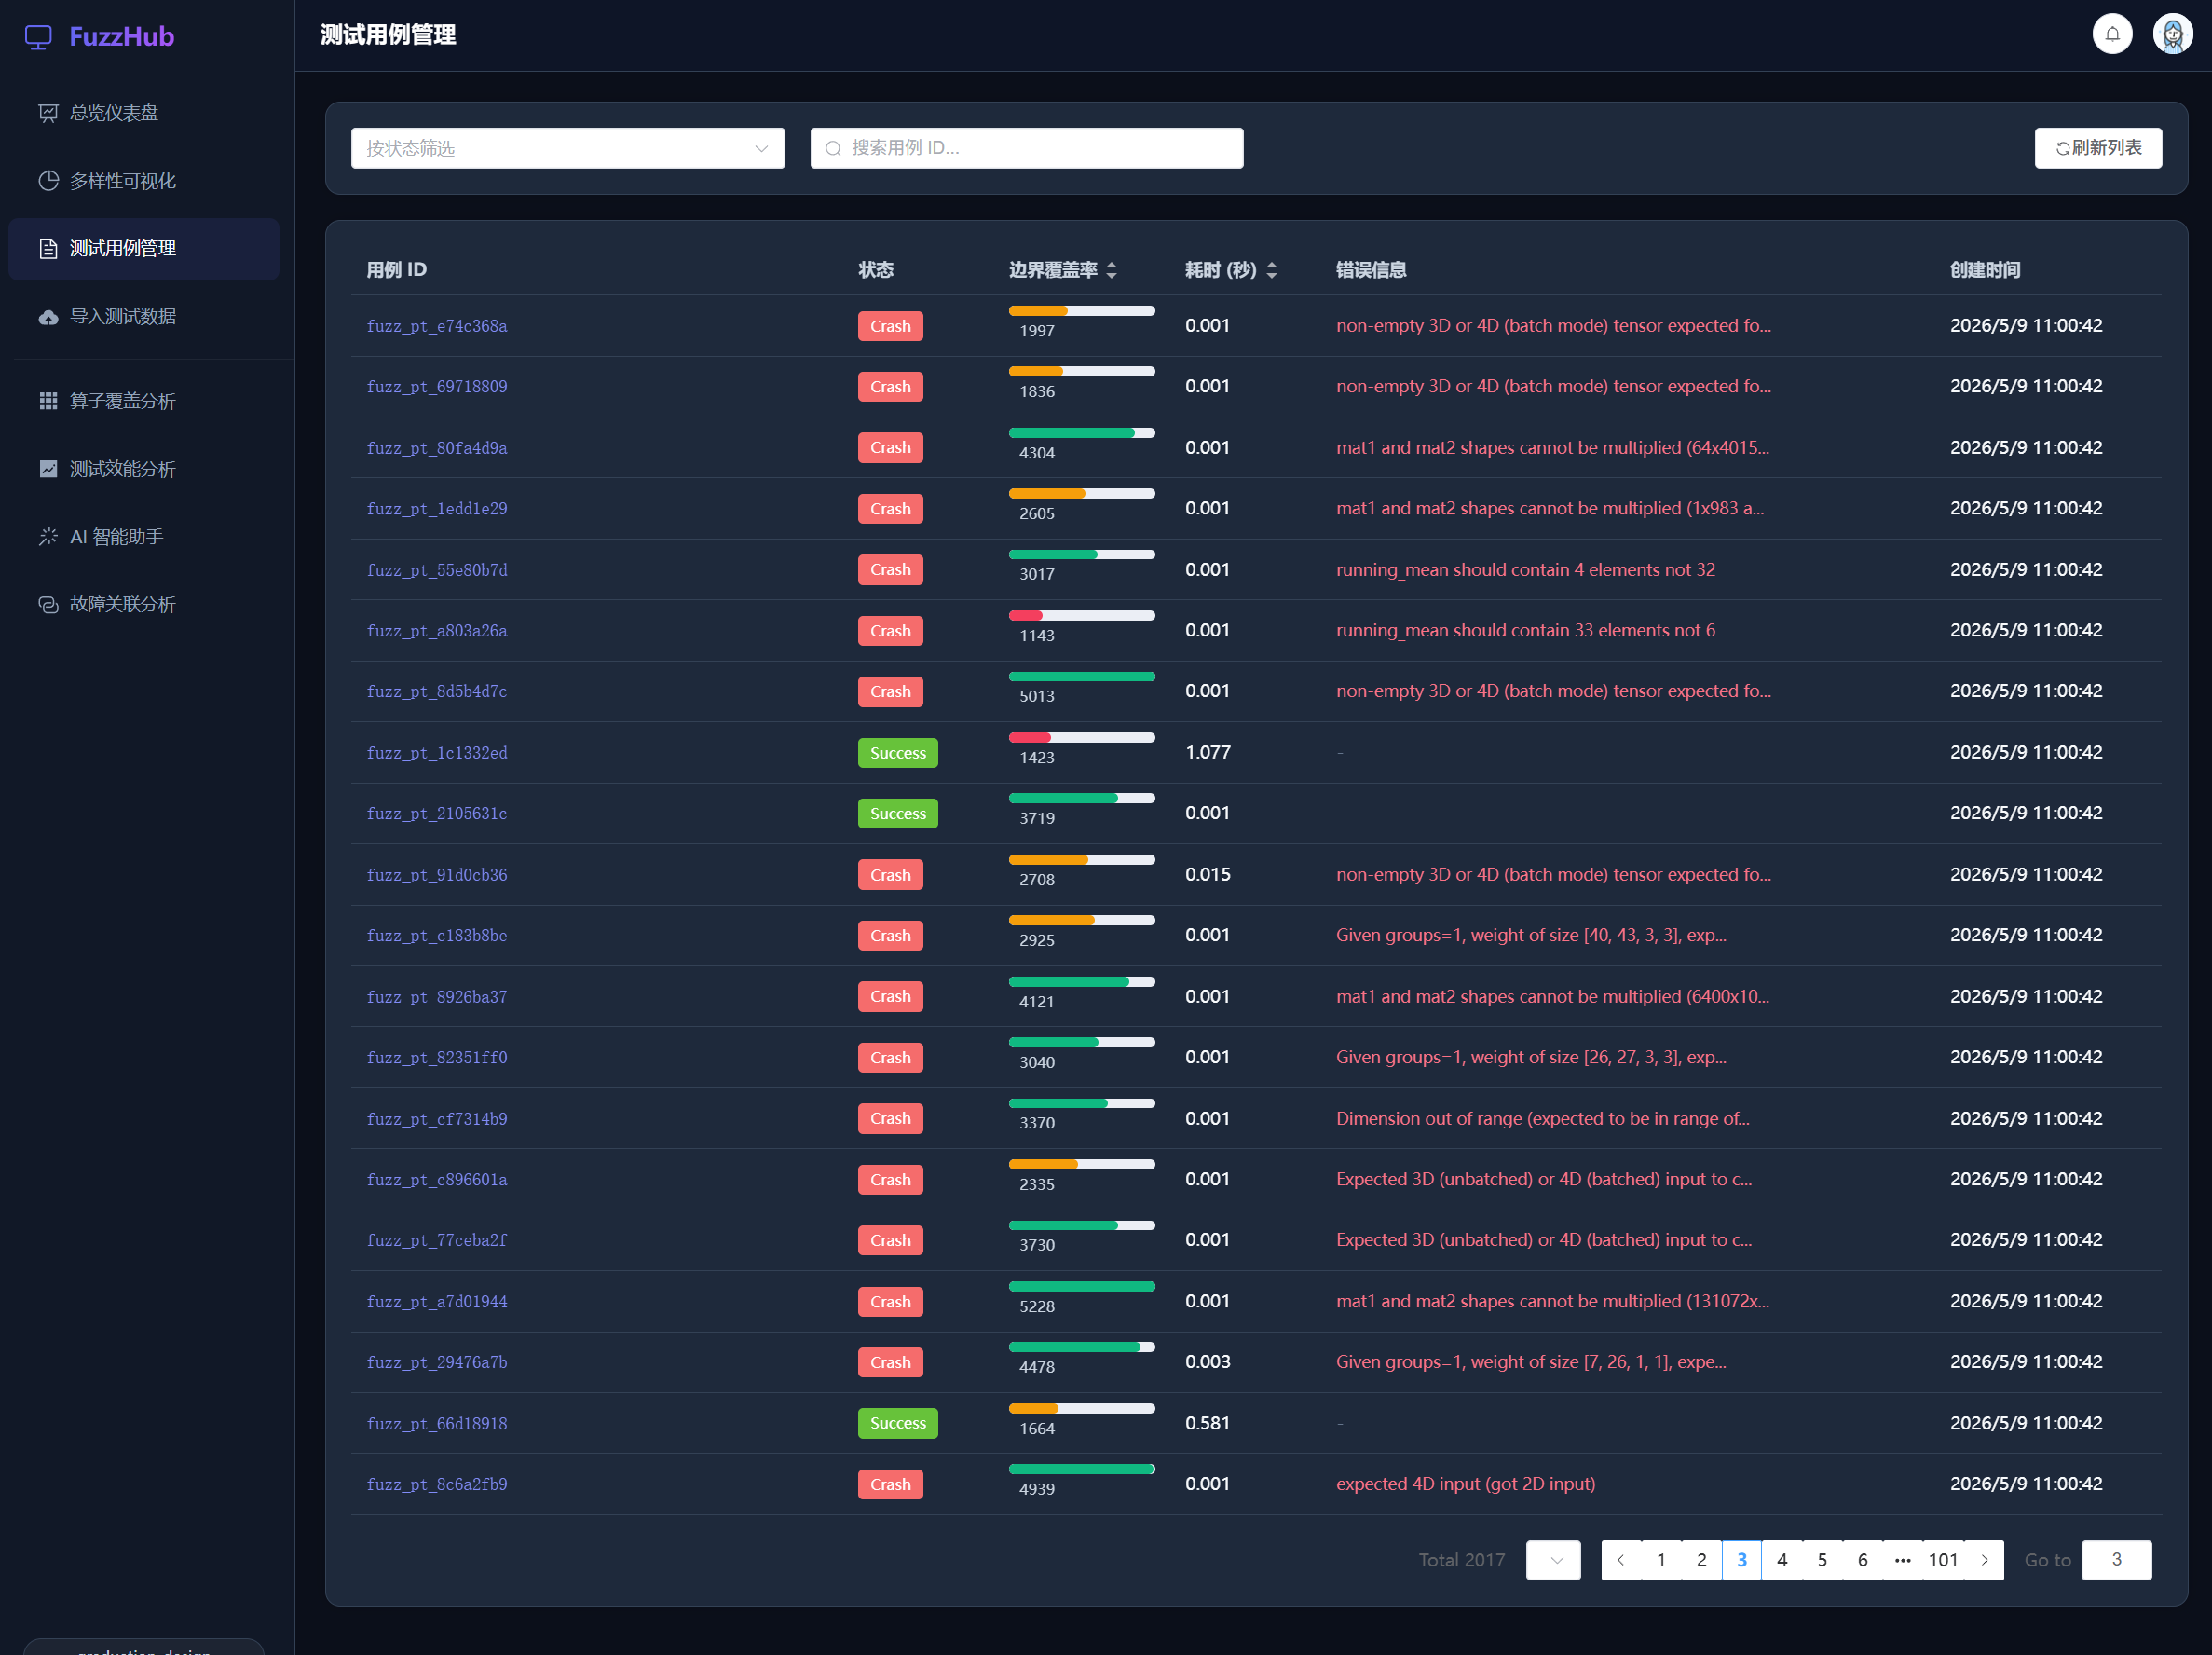
\includegraphics[width=0.75\textwidth]{figure/ui_sample_manage.png}
\caption{测试用例管理界面}
\label{fig:ui_sample_manage}
\end{figure}
\FloatBarrier

\subsection{用例详情故障辅助定位界面}

用例详情界面用于展示单条测试用例的完整信息。
除用例ID、执行状态、运行耗时和覆盖数据外，
页面还会展示错误日志、模型结构和输入参数等内容。
对于失败用例，前端会调用Python后端分析接口，
给出错误类别、候选算子节点和相关说明，
帮助用户缩小排查范围。

该界面还提供候选边界条件分析入口。
用户可以针对某个失败用例发起候选边界条件分析，
查看成功用例与失败用例之间的参数差异，
并生成满足或不满足候选约束的待人工验证样例。
用例详情故障辅助定位界面如图\ref{fig:ui_fault_location}所示。

\begin{figure}[htbp]
\centering
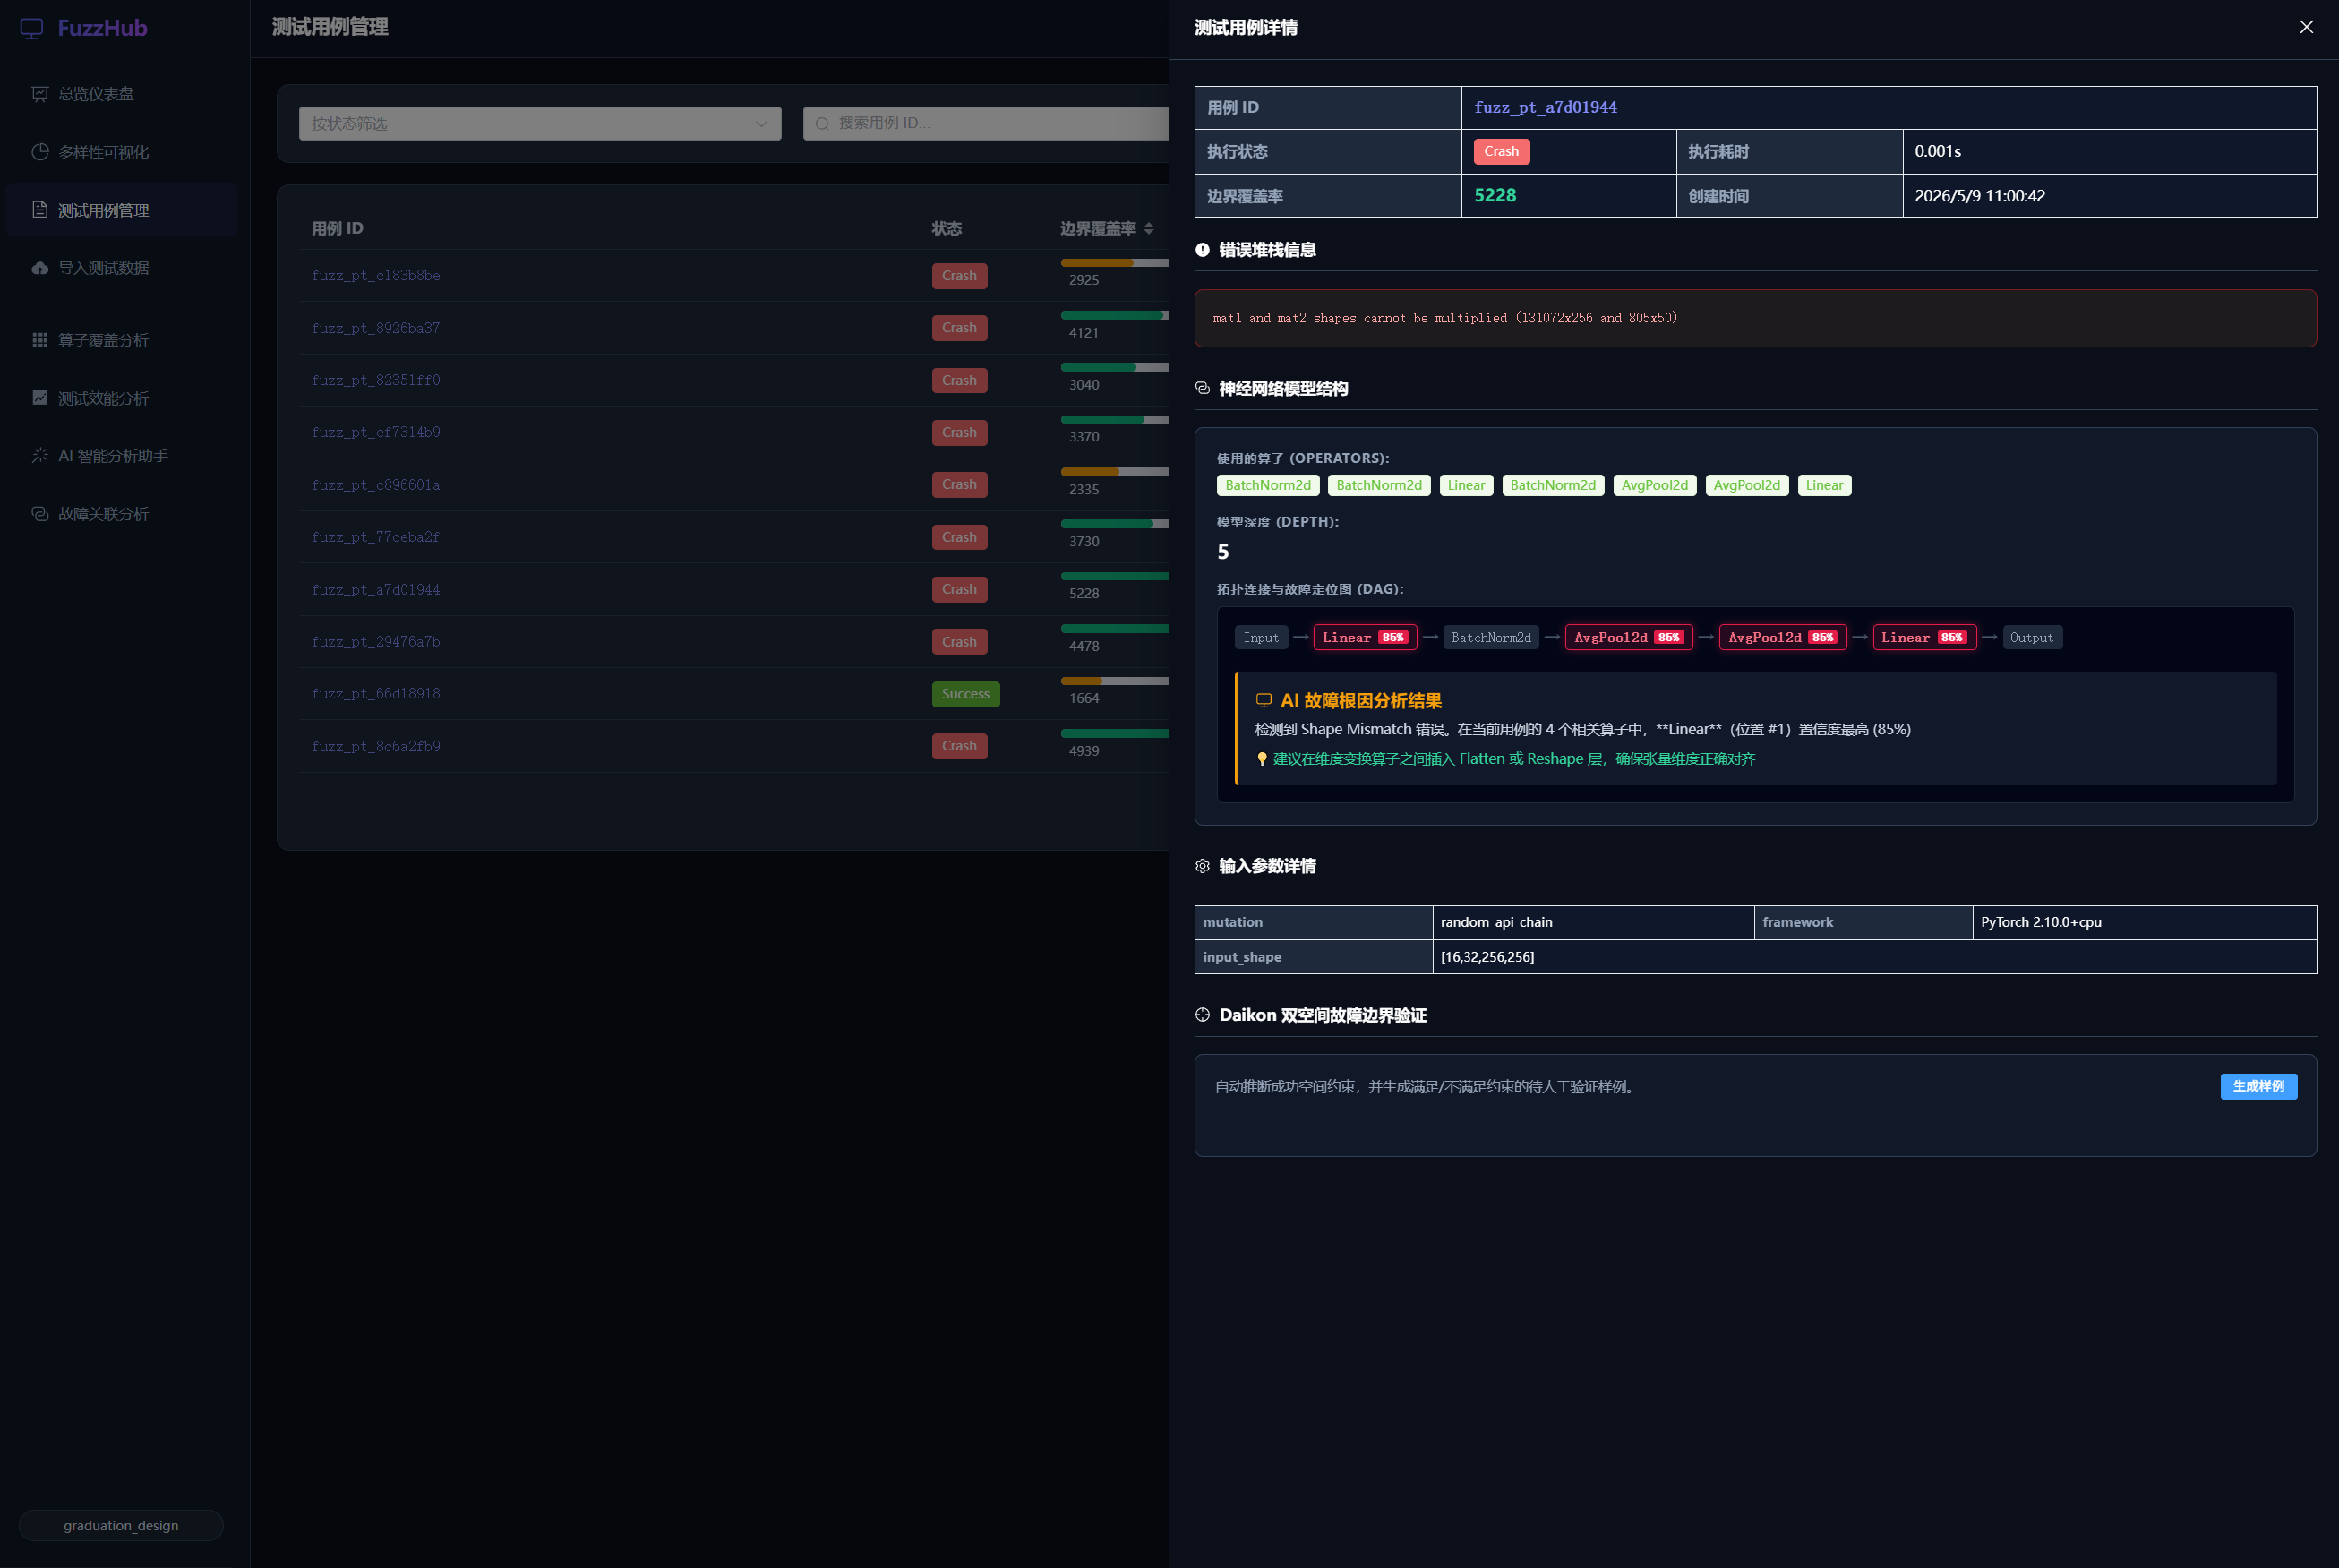
\includegraphics[width=0.75\textwidth]{figure/ui_fault_location.png}
\caption{用例详情故障辅助定位界面}
\label{fig:ui_fault_location}
\end{figure}
\FloatBarrier

\subsection{AI智能分析助手界面}

AI智能分析助手页面用于提供自然语言查询和辅助分析功能。
用户输入问题后，系统会结合历史测试用例进行语义检索，
并生成辅助诊断报告。
页面同时展示相似用例、错误摘要和候选变异建议，
方便用户从已有数据中寻找参考。

该页面主要调用语义问答接口和建议生成接口。
其中，前者用于组织历史相似用例和当前问题上下文，
后者用于给出后续测试方向。
用于辅助开发者进行故障分析和后续测试。
AI智能分析助手界面如图\ref{fig:ui_ai_assistance}所示。

\begin{figure}[htbp]
\centering
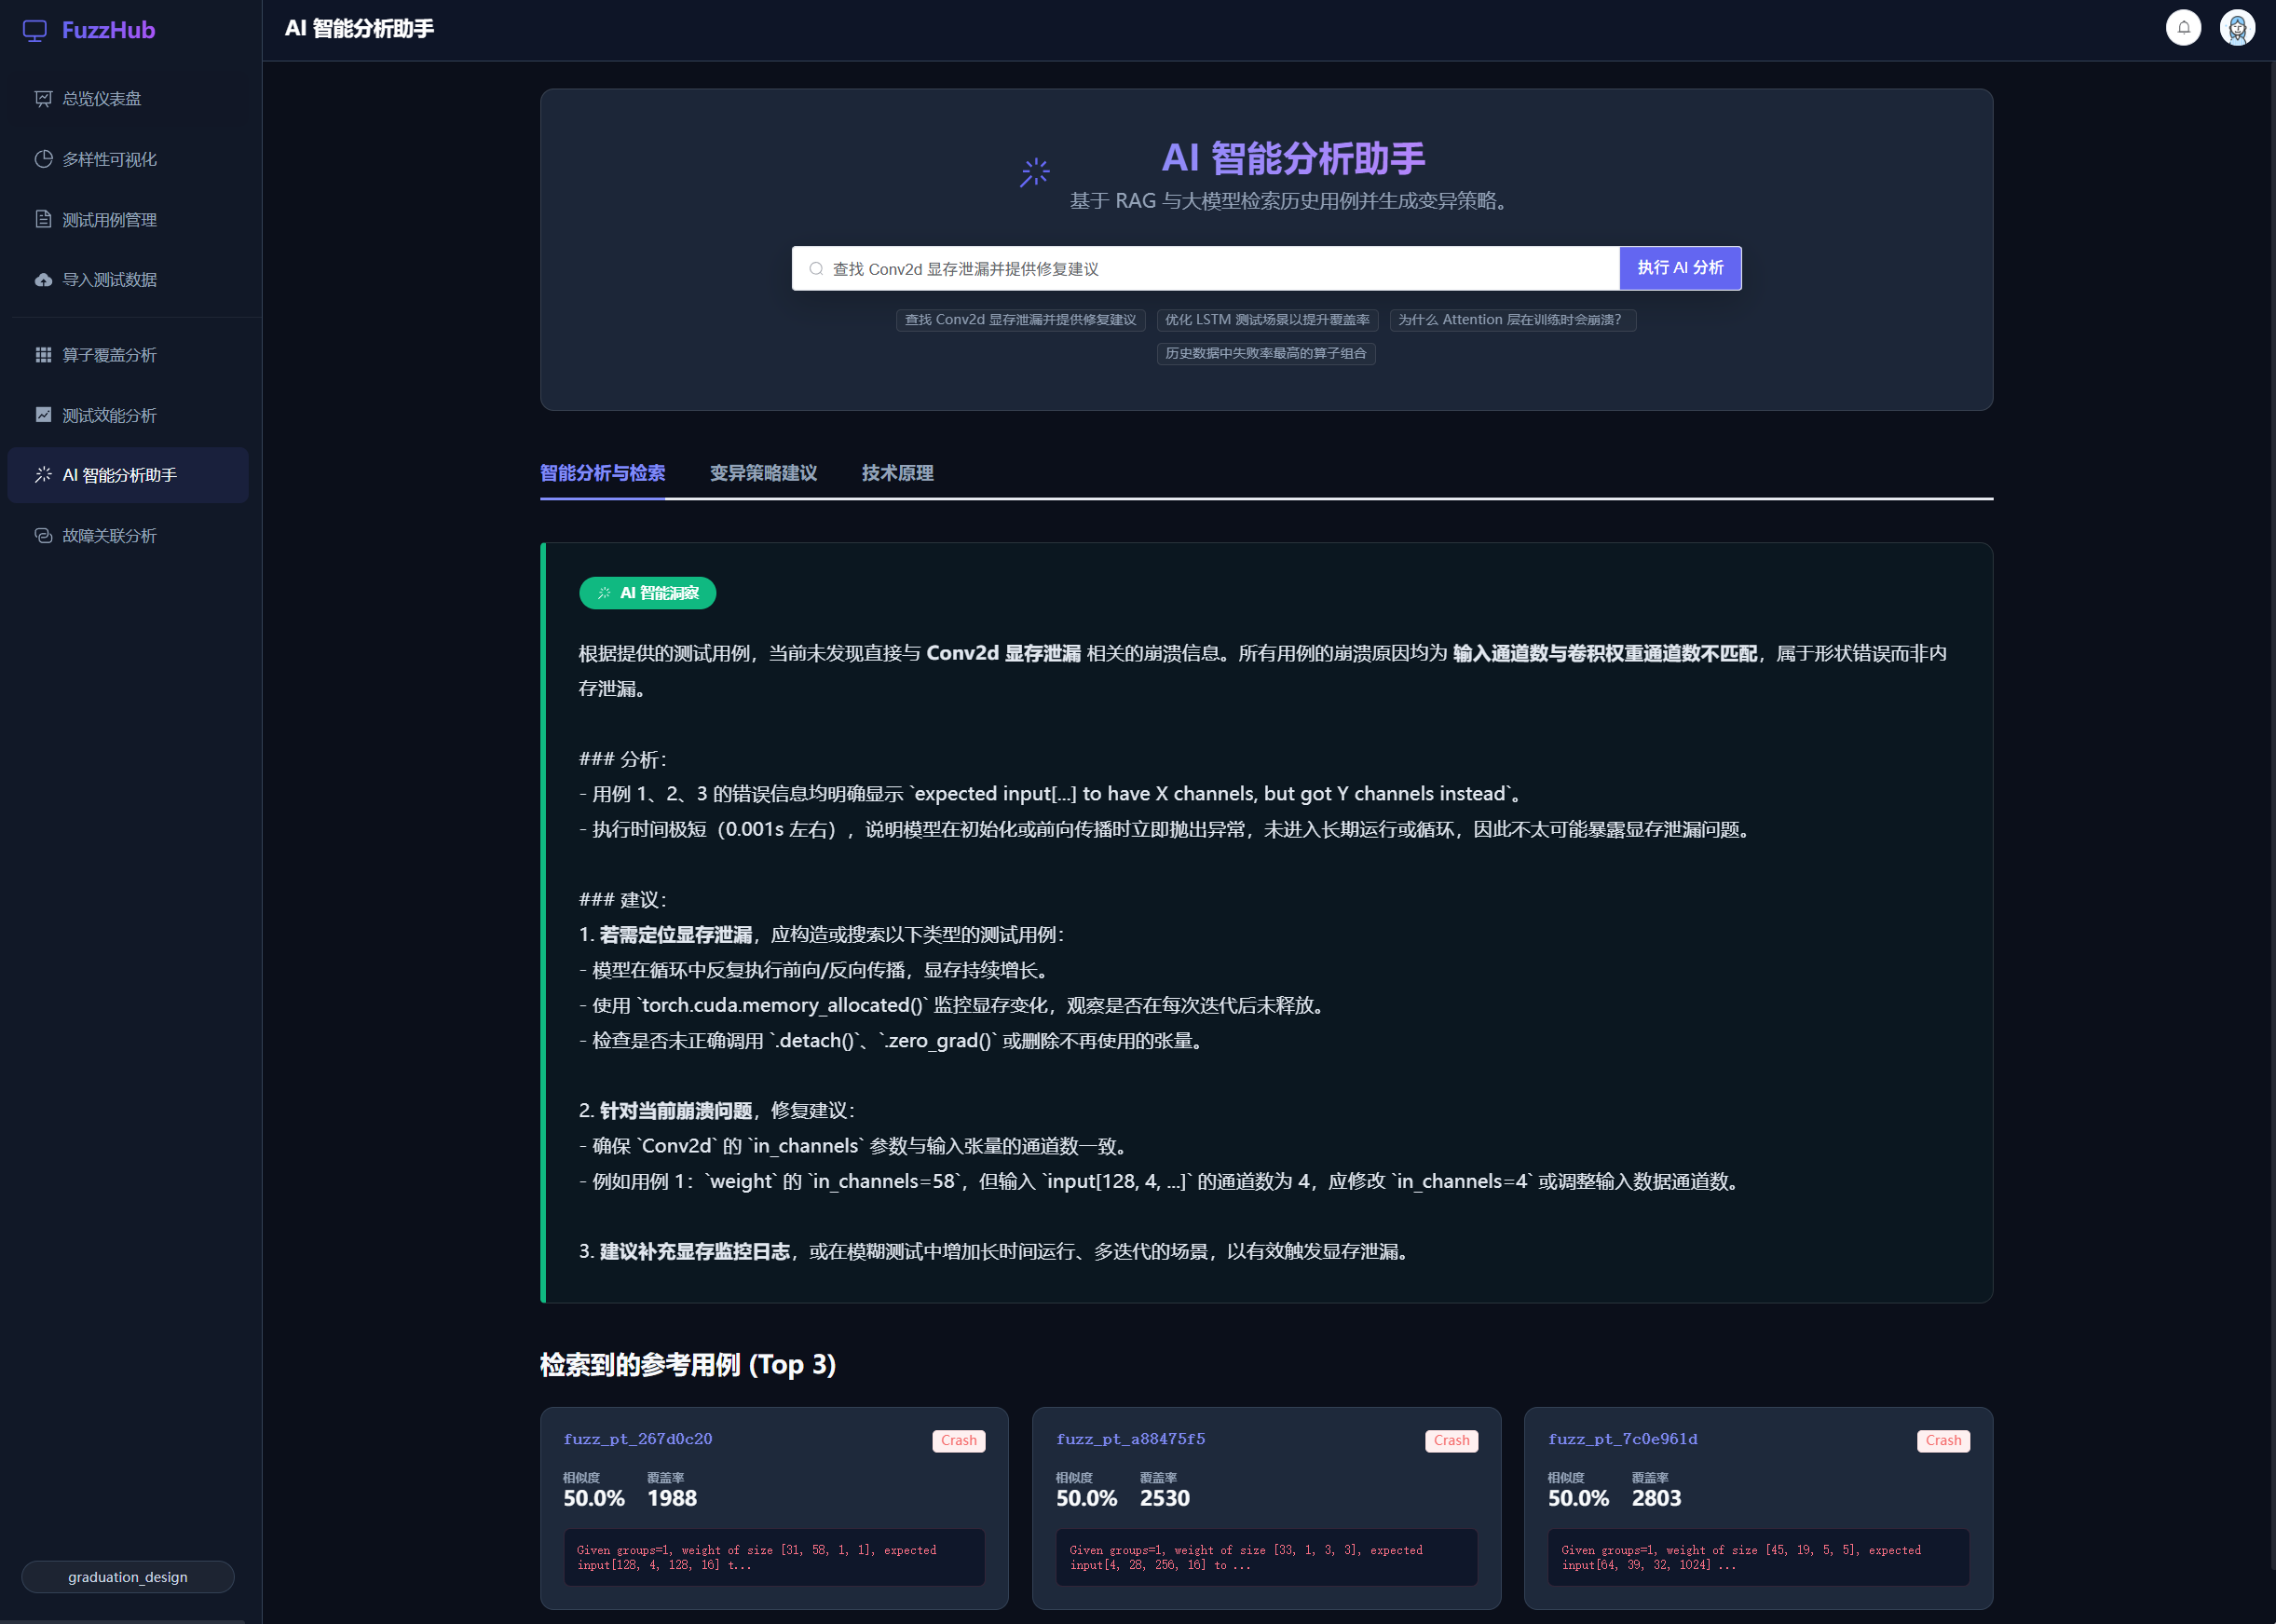
\includegraphics[width=0.75\textwidth]{figure/ui_ai_assistance.png}
\caption{AI智能分析助手界面}
\label{fig:ui_ai_assistance}
\end{figure}
\FloatBarrier

\subsection{故障关联分析界面}

故障关联分析页面用于从整体上查看故障与算子的关系。
页面根据后端返回的故障关联数据，
展示故障用例数量、高风险算子关联和常见错误类型。
中部表格按算子和算子组合汇总故障情况，
便于观察问题是否集中在某些算子或特定连接关系上。
页面还列出部分个案级故障记录，
用户可以从中选择失败用例继续进行边界对比分析。
“故障关联分析”页面如图\ref{fig:ui_fault_analysis}所示。

\begin{figure}[htbp]
\centering
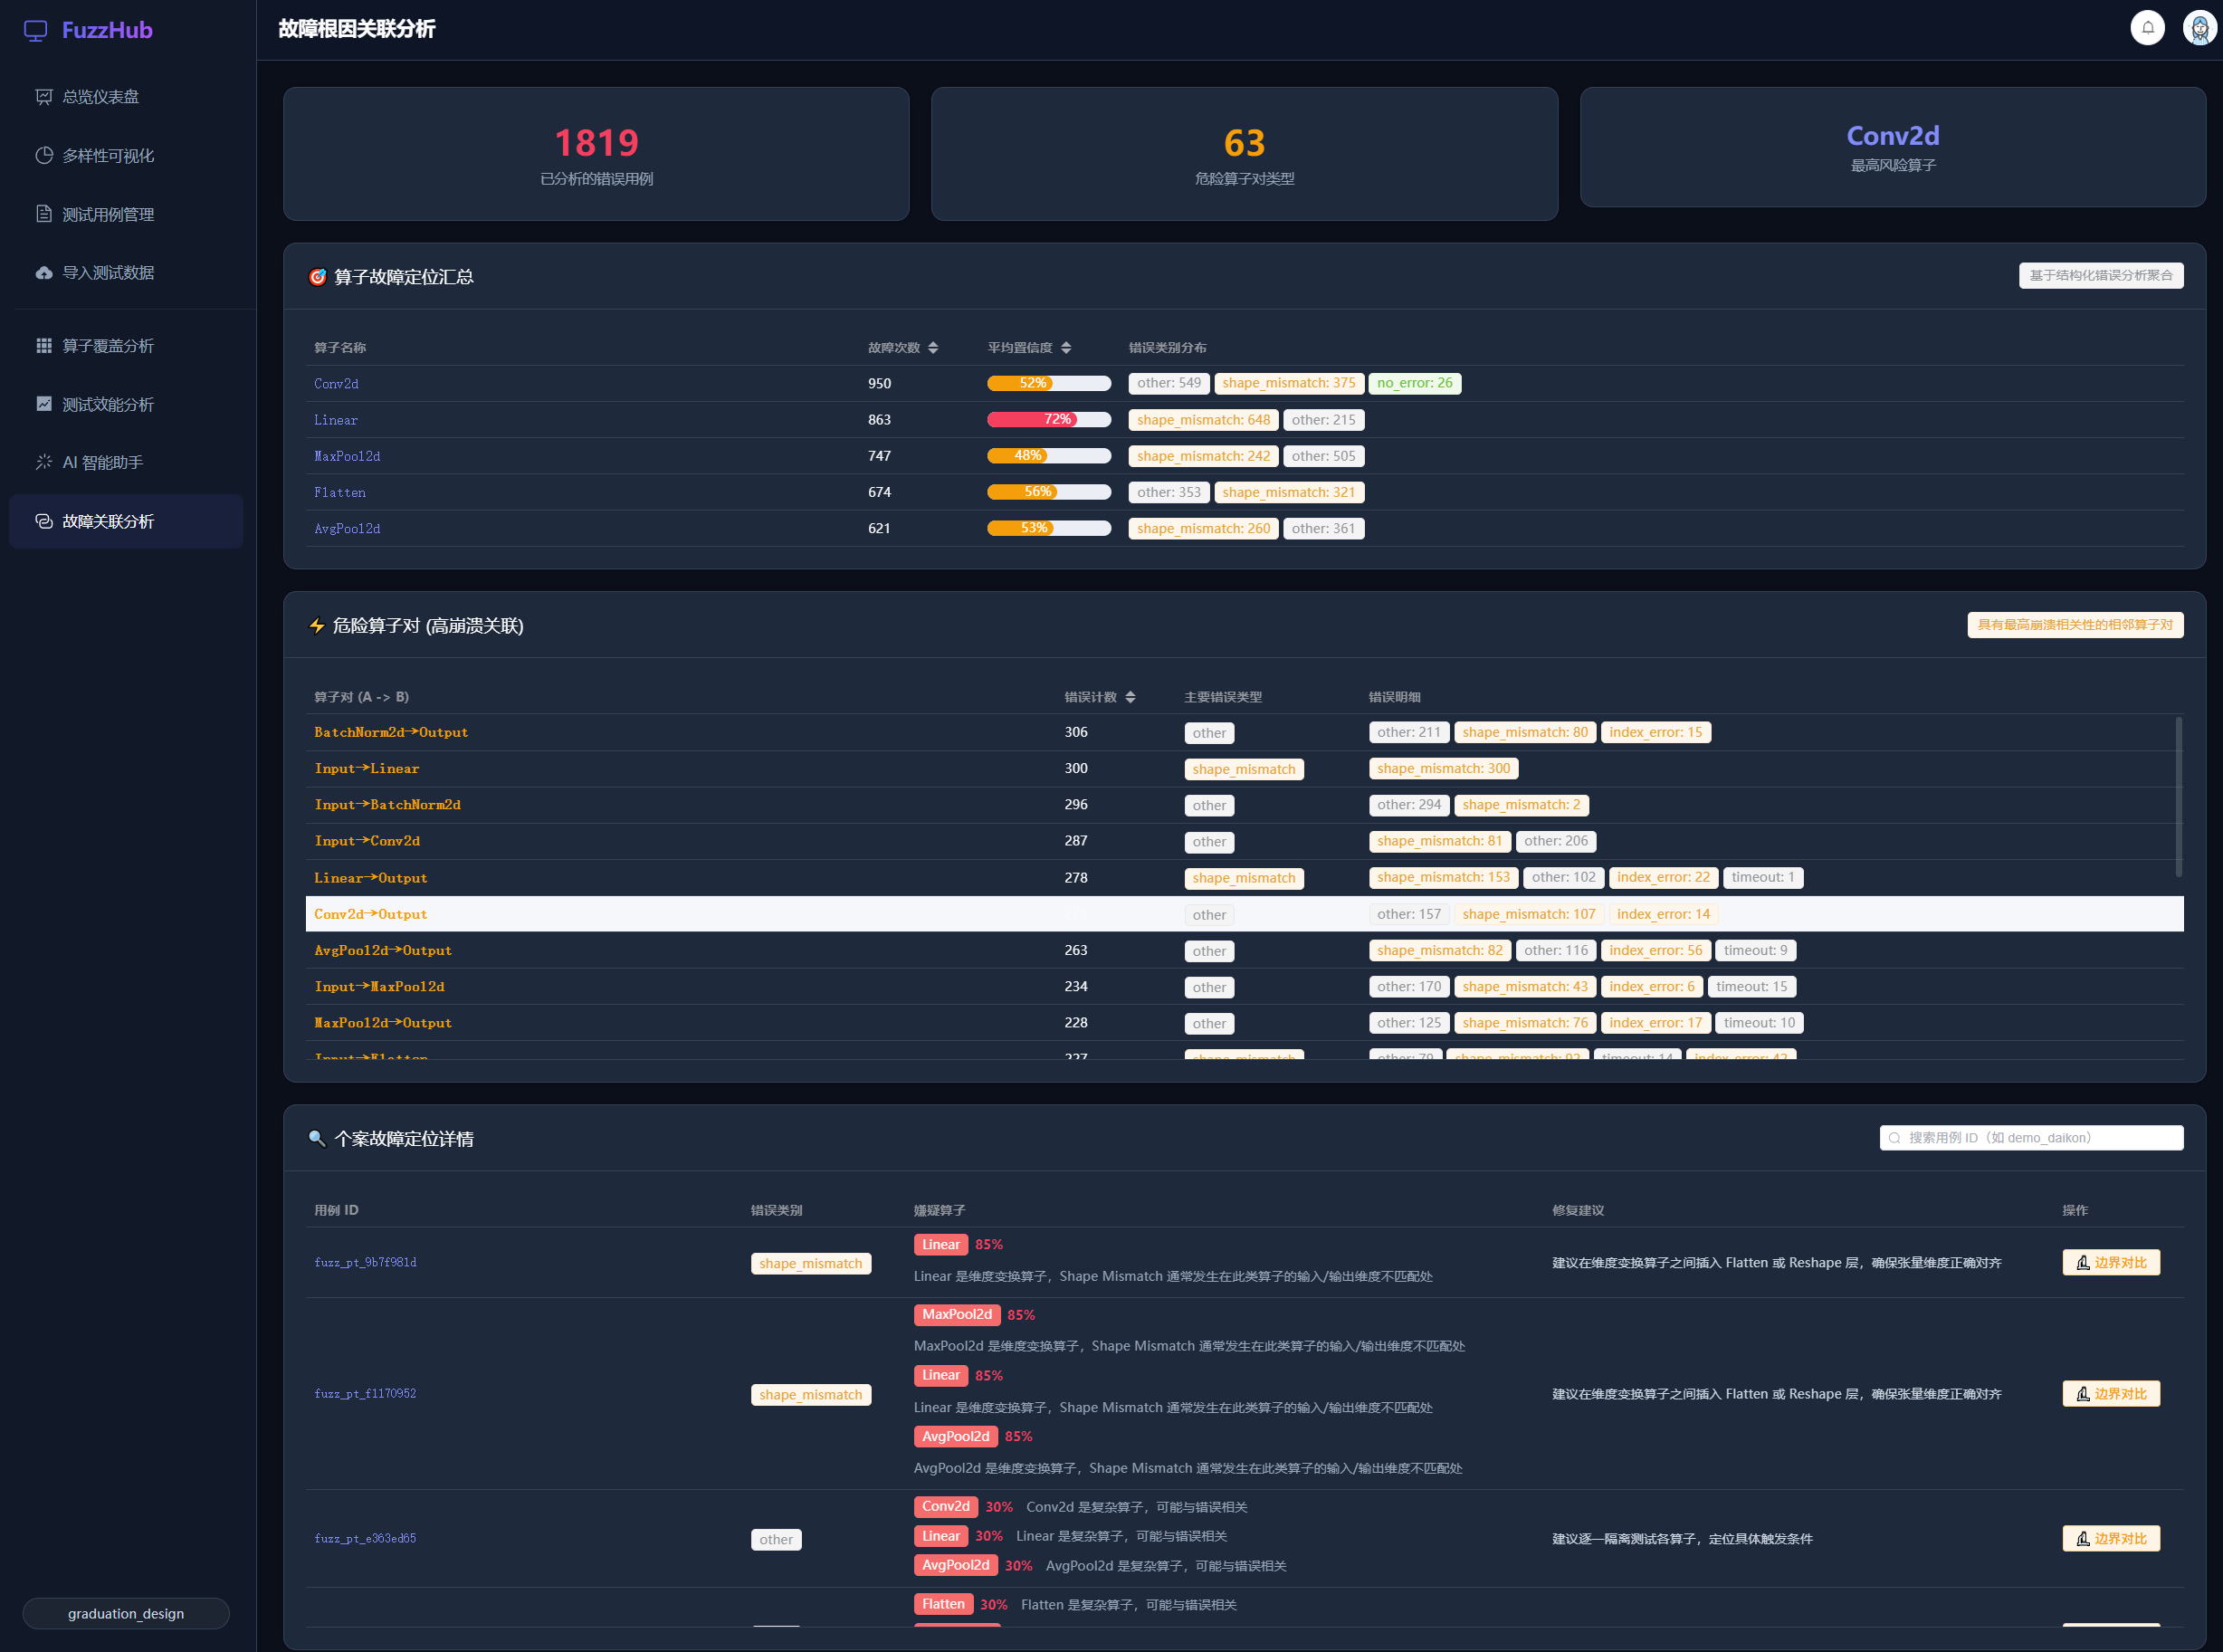
\includegraphics[width=0.75\textwidth]{figure/ui_fault_analysis.png}
\caption{故障关联分析}
\label{fig:ui_fault_analysis}
\end{figure}

边界对比弹窗用于展示单个失败用例与相近成功用例之间的差异。
弹窗中同时展示参数差分、Daikon候选约束、验证样例和辅助诊断报告。
其中，候选约束用于提示可能存在的参数边界，
验证样例则分为满足约束和违反约束两类，
作为后续补充测试和验证边界条件的参考。
界面会标记这些样例仍处于待人工验证状态，
避免把生成结果直接解释为已经执行通过或失败。
底部的辅助诊断报告用于解释候选边界条件。
故障临界差分对比弹窗如图\ref{fig:ui_daikon}所示。

\begin{figure}[htbp]
\centering
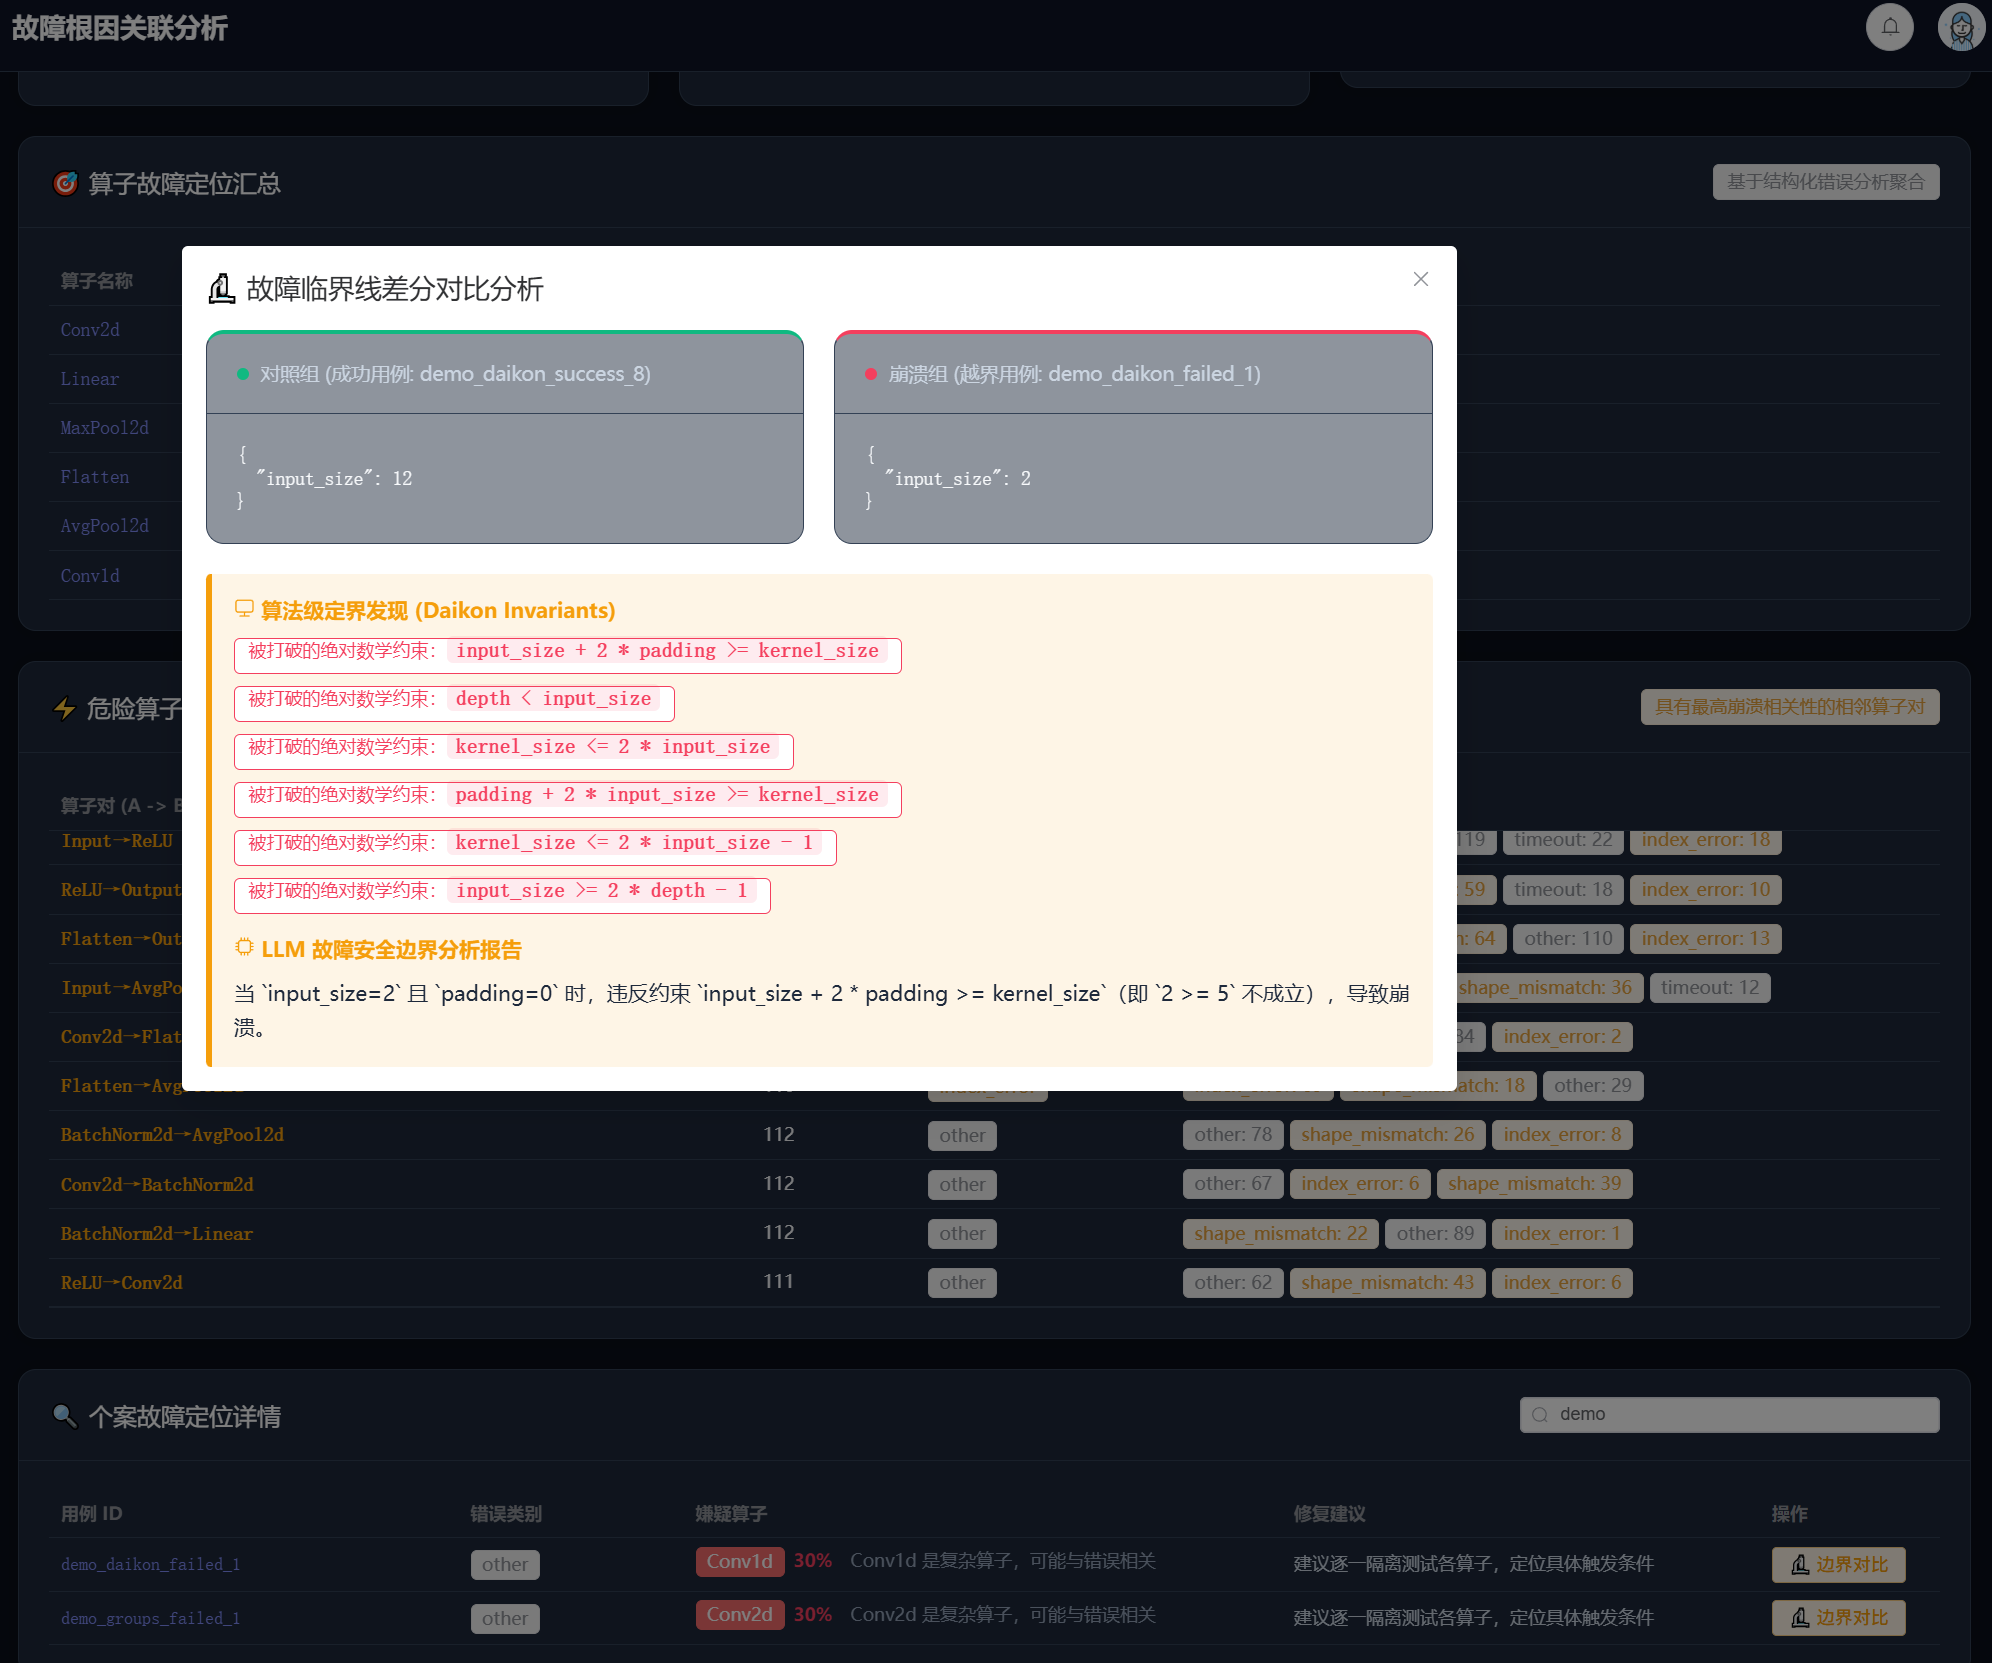
\includegraphics[width=0.75\textwidth]{figure/ui_daikon.png}
\caption{故障临界差分对比}
\label{fig:ui_daikon}
\end{figure}
\FloatBarrier

\subsection{算子覆盖缺口分析界面}

算子覆盖缺口分析页面用于查看当前测试集对算子和算子组合的覆盖情况。
页面通过覆盖缺口分析接口获取统计结果，
并以统计卡片、热力图和表格的形式展示。
用户可以看到哪些算子已经被测试覆盖，
哪些算子对在现有用例中还没有出现。
这部分信息为后续补充测试提供了直接依据。
算子覆盖缺口分析界面如图\ref{fig:ui_coverage}所示。

\begin{figure}[htbp]
\centering
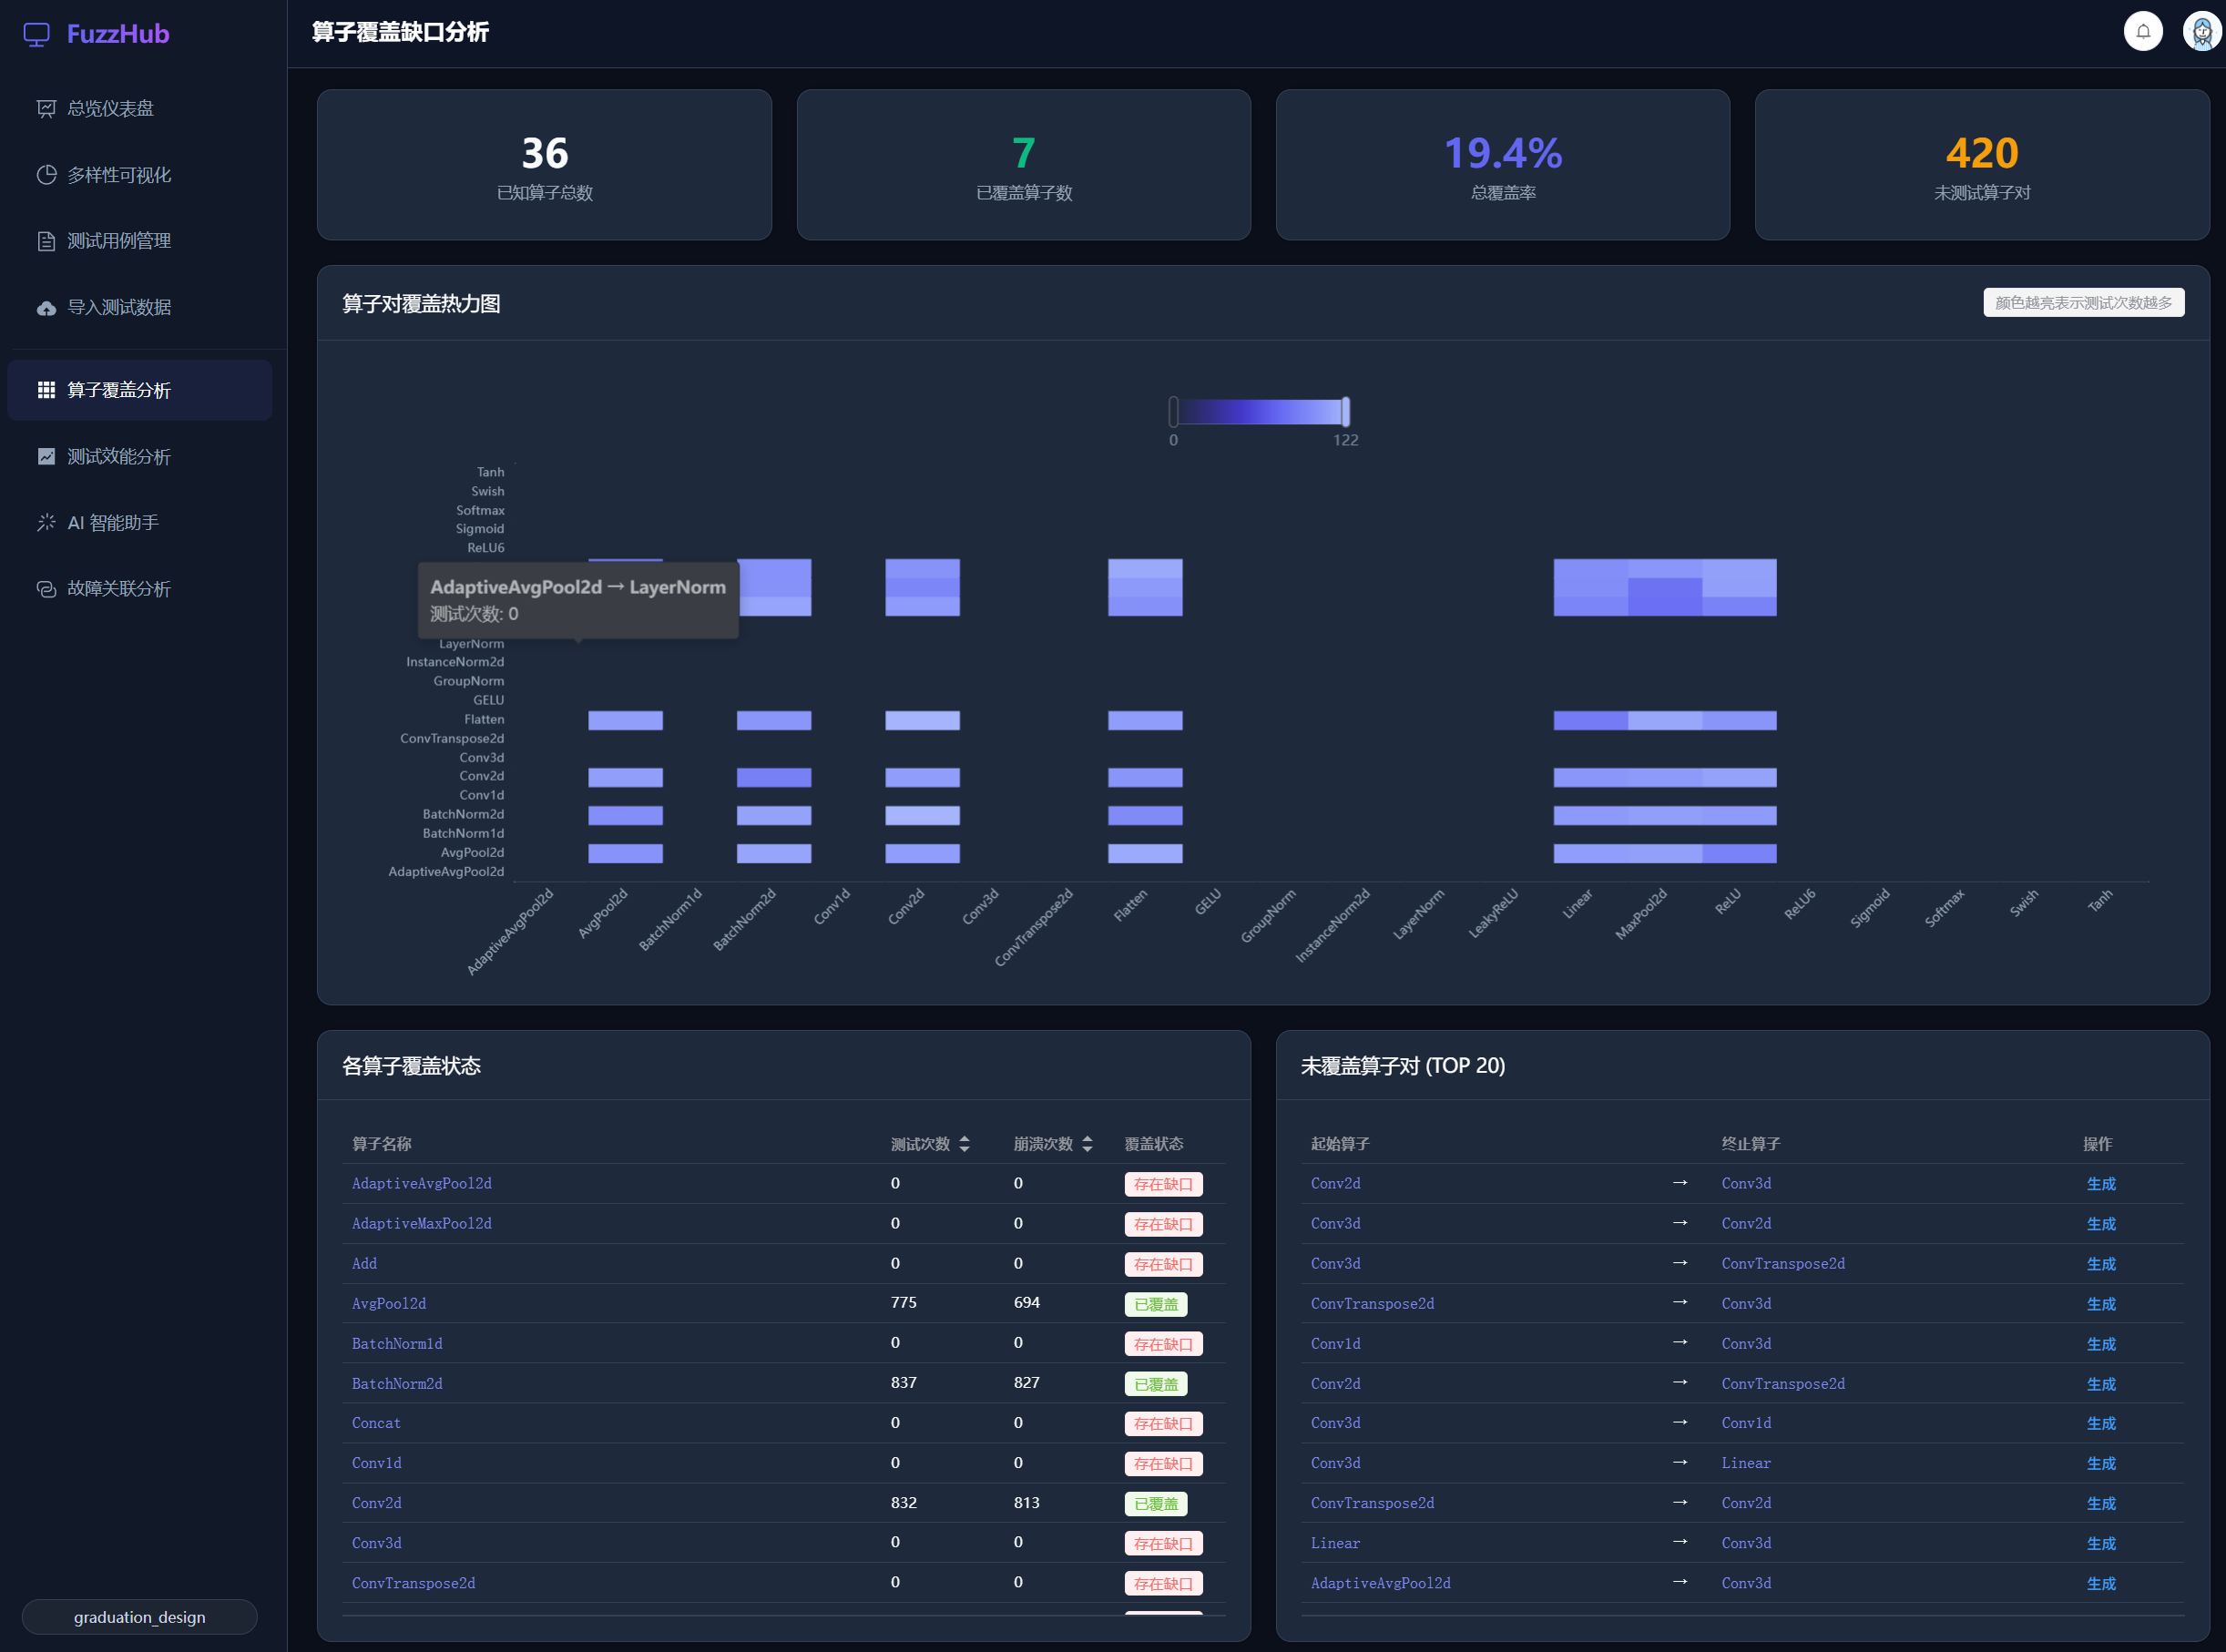
\includegraphics[width=0.75\textwidth]{figure/ui_coverage.png}
\caption{算子覆盖缺口分析界面}
\label{fig:ui_coverage}
\end{figure}

对于未覆盖的算子组合，页面提供候选补盲测试脚本生成入口。
用户选择目标算子对后，
前端调用候选补盲生成接口生成候选脚本。
生成结果会在弹窗中展示，
用户可以据此检查脚本是否可运行、是否具有覆盖贡献以及是否适合后续入库。
AI定向补盲生成结果界面如图\ref{fig:ui_coverage_blind}所示。

\begin{figure}[htbp]
\centering
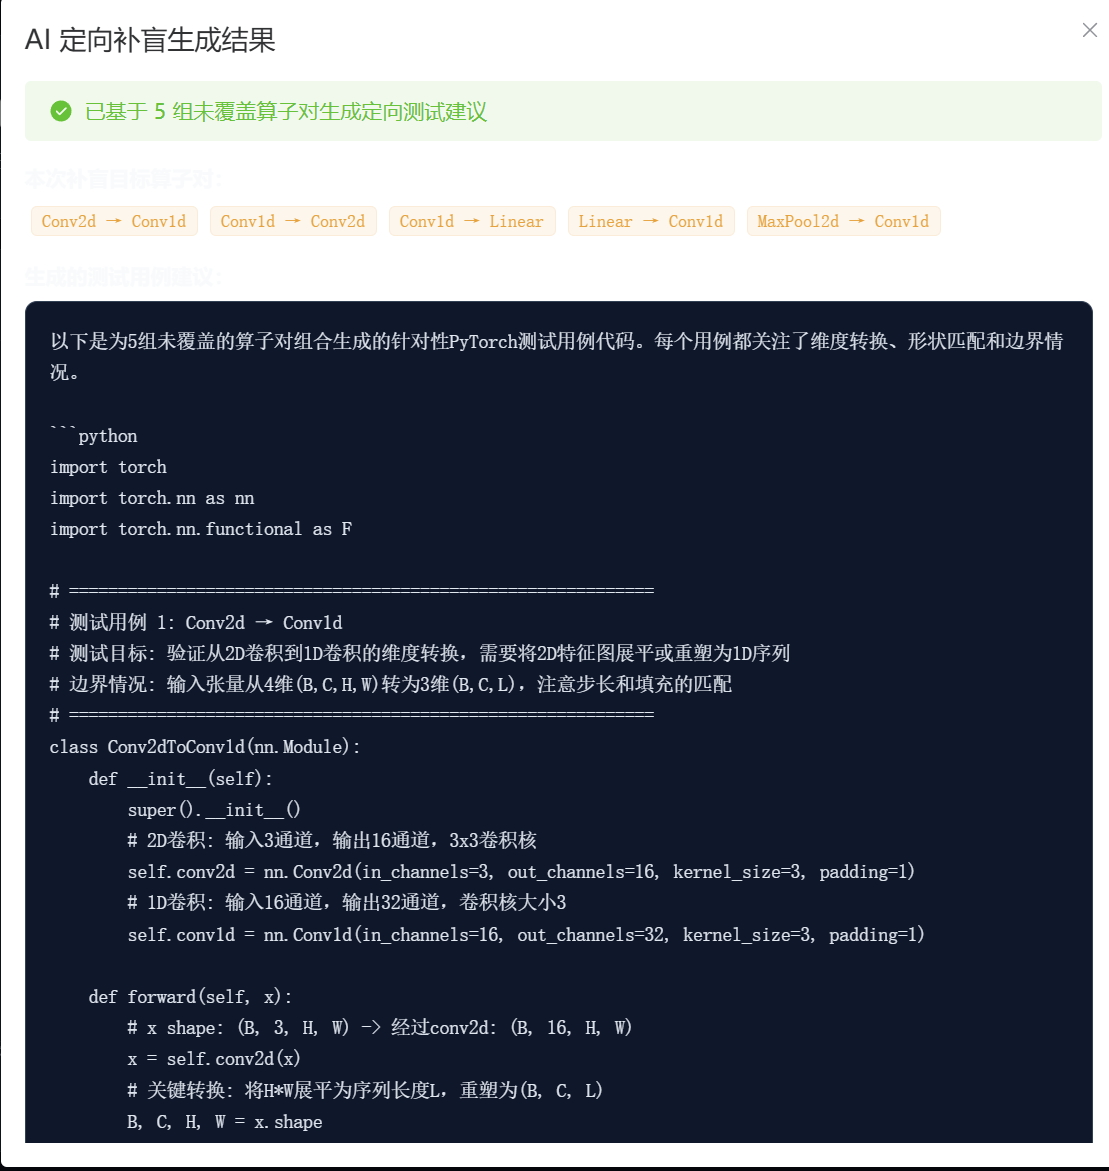
\includegraphics[width=0.75\textwidth]{figure/ui_coverage_blind.png}
\caption{AI定向补盲生成结果界面}
\label{fig:ui_coverage_blind}
\end{figure}
\FloatBarrier

\subsection{测试效能评估界面}

测试效能评估页面用于展示CEI指标、用例效能排行和清退方案，
帮助用户区分优先保留用例和候选清退用例。
用户可以先预览阈值清退结果，确认后再执行处理。
测试效能评估界面如图\ref{fig:ui_efficiency_scatter}所示。

\begin{figure}[H]
\centering
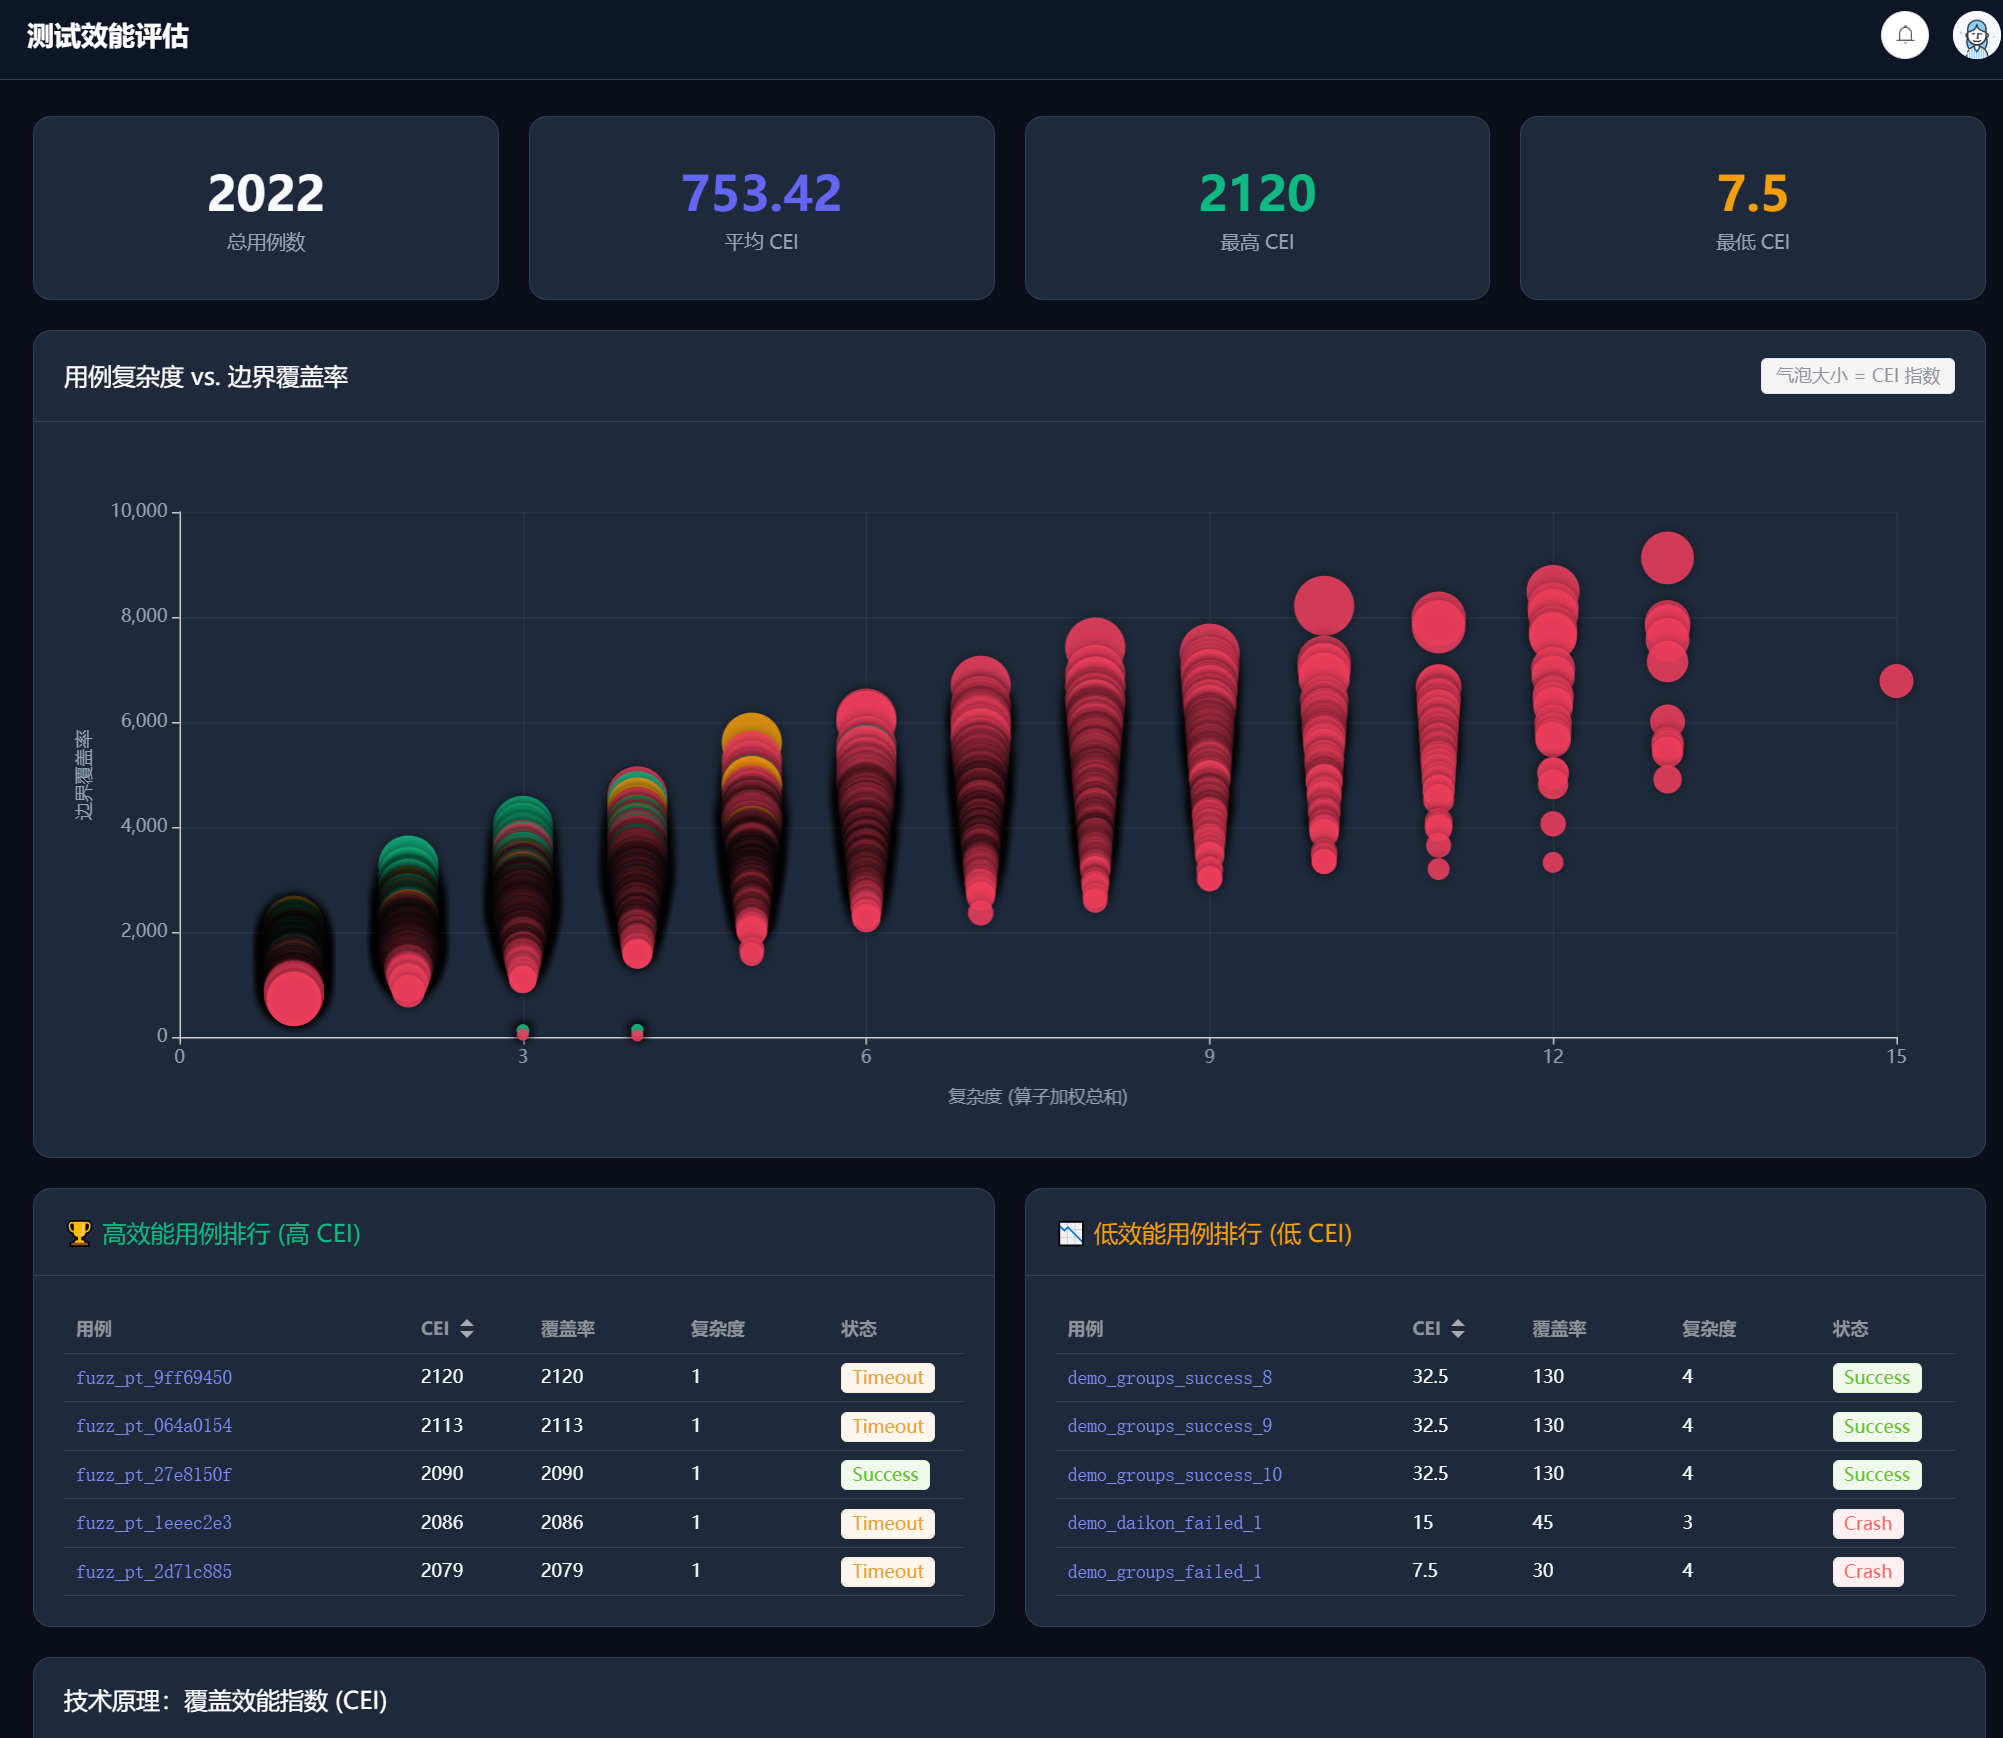
\includegraphics[width=0.75\textwidth]{figure/ui_efficiency_scatter.png}
\caption{测试效能评估界面}
\label{fig:ui_efficiency_scatter}
\end{figure}
\FloatBarrier

\subsection{测试用例多样性分布界面}

多样性分析页面用于展示测试用例在二维PCA投影空间中的分布情况。
页面通过散点图展示不同执行状态的样例位置，
帮助用户从整体上观察测试集是否过于集中。
如果大量样例聚集在少数区域，
说明当前测试数据可能偏向少量模型结构或错误模式；
如果部分区域较稀疏，
则可以作为后续补充测试和构造候选补盲测试脚本的参考。
测试用例多样性分布界面如图\ref{fig:ui_diversity}所示。

\begin{figure}[htbp]
\centering
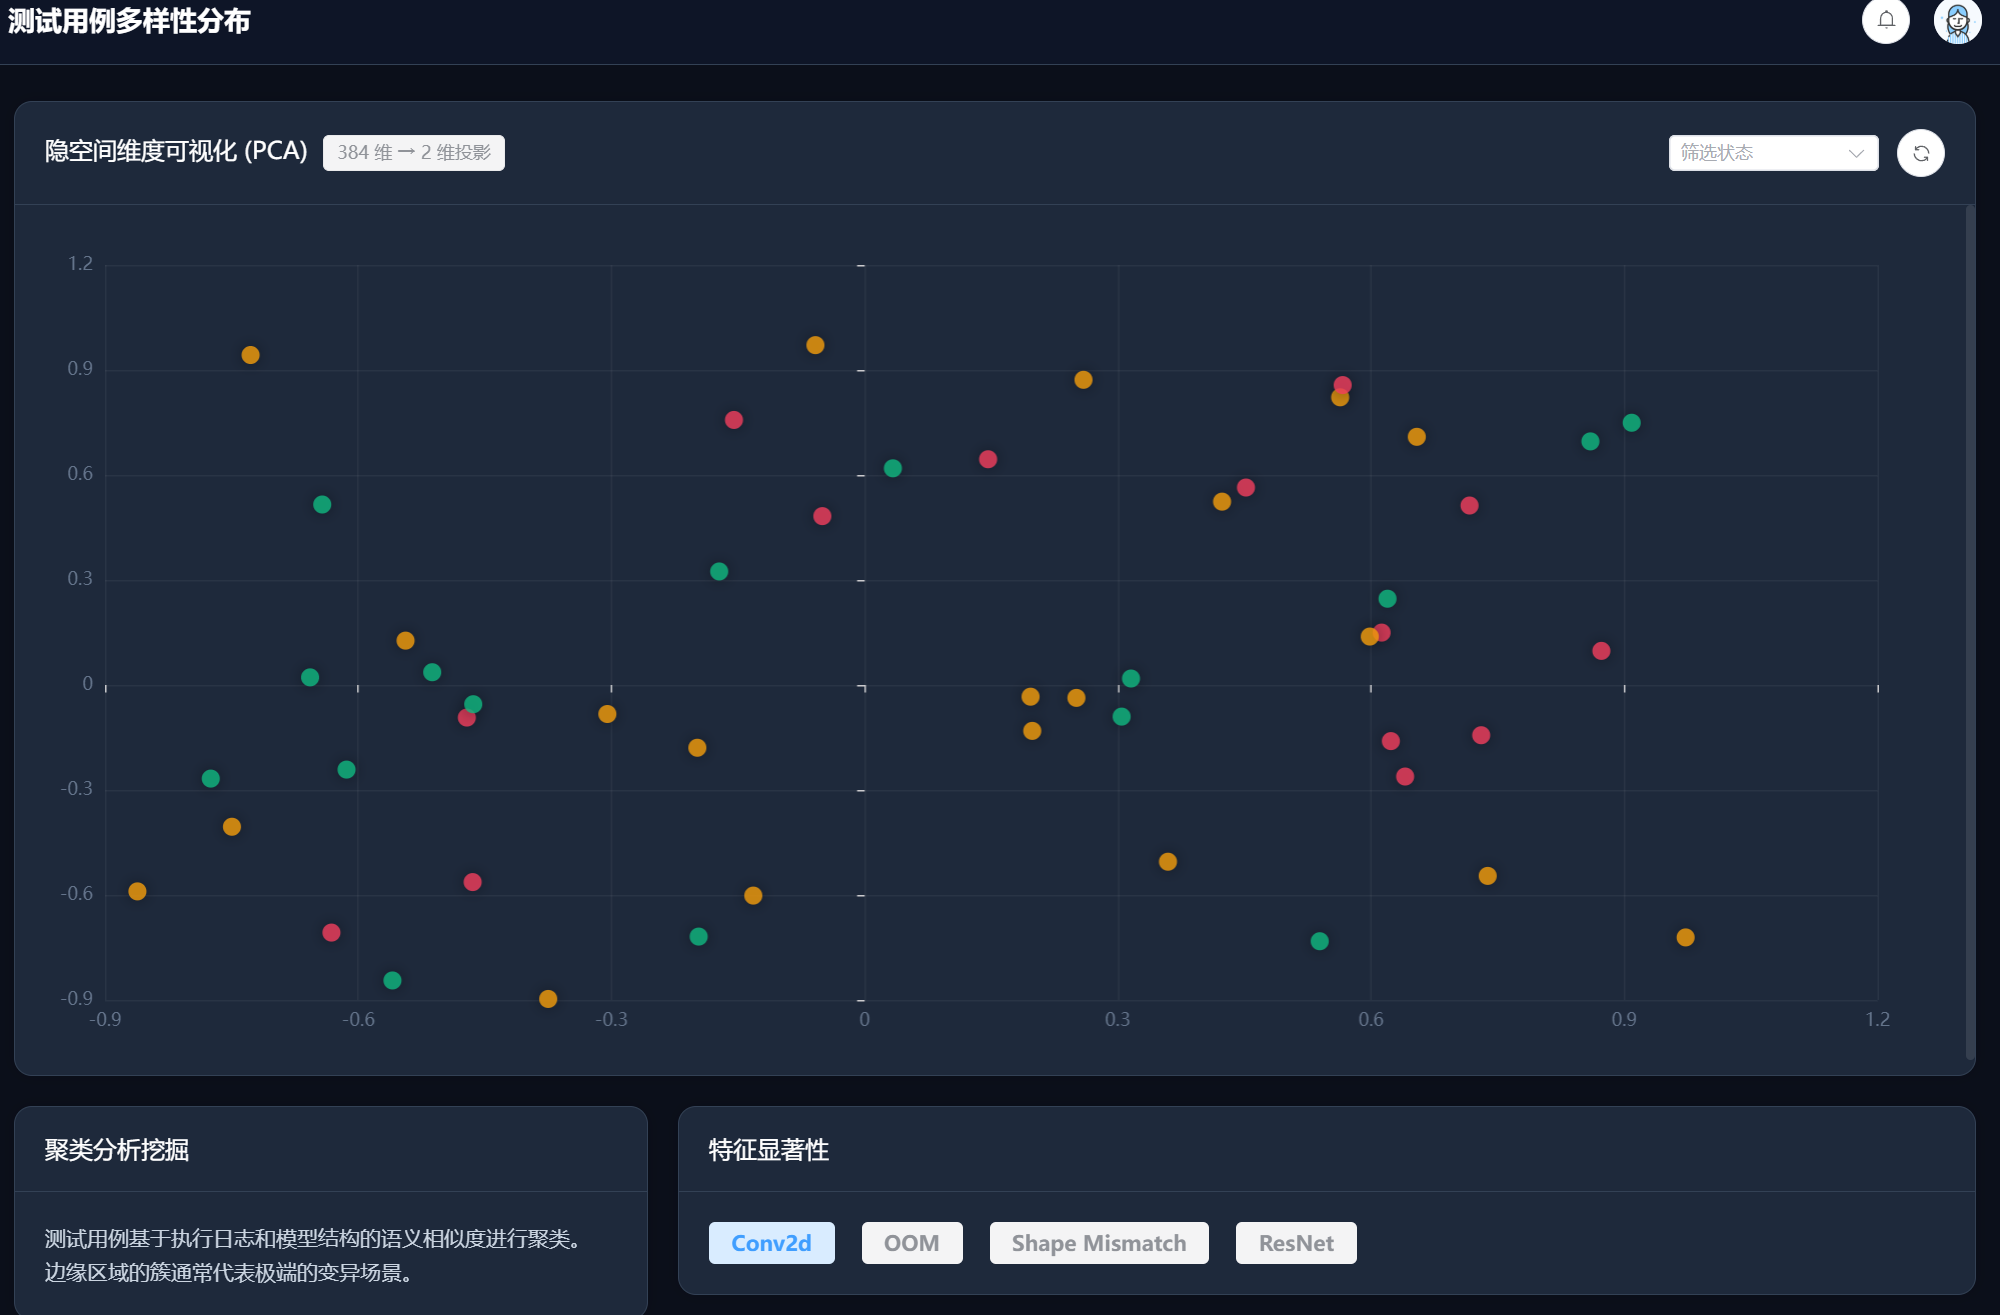
\includegraphics[width=0.75\textwidth]{figure/ui_diversity.png}
\caption{测试用例多样性分布}
\label{fig:ui_diversity}
\end{figure}
\FloatBarrier
